\documentclass[12pt, a4paper, twoside, openright, english]{book}

\usepackage[english]{babel}
\usepackage[utf8]{inputenc}
\usepackage[T1]{fontenc}
\usepackage[top=2.5cm,
	bottom=3cm,
	right=3.2cm,
	left=3.2cm
]{geometry}

\usepackage{subcaption}
\usepackage{hyperref}
\usepackage{enumitem}
\usepackage{tabularx}
\usepackage{afterpage}
\usepackage{longtable}
\usepackage{multirow}
\usepackage{amsfonts}
\usepackage{amssymb}
\usepackage{listings}
\usepackage{titlesec}
\usepackage{setspace}
\usepackage{fancyhdr}
\usepackage{fancyvrb}
\usepackage[fleqn]{amsmath}
\usepackage{pdfpages}
\usepackage{nccmath}
\usepackage{csquotes}
\usepackage{diagbox}
\usepackage{ifthen}
\usepackage{algorithm}
\usepackage{mathabx}
\usepackage{algpseudocode}
\usepackage[super]{nth}

\usepackage[titles]{tocloft} % TOC header same as chapter title
%\usepackage{showframe}
\usepackage{titlesec}
\titlespacing*{\chapter}{0pt}{0pt}{40pt}

\usepackage{colortbl}
\usepackage{tabulary}
\usepackage{adjustbox}

\usepackage{lmodern}
\usepackage{fourier-orns}
\newlength\longest

% Abbreviations
\usepackage{nomencl}
\makenomenclature
\renewcommand{\nomname}{List of Abbreviations}


\usepackage{expl3}
\usepackage{etoolbox}
%\preto\tabular{\shorthandoff{-}}

\usepackage[style=iso-numeric, backend=biber, url=false]{biblatex}
\renewcommand*{\bibfont}{\normalfont\small}
\addbibresource{literature.bib}


% Formulas
\newcommand{\listequationsname}{List of Equations}
\newlistof{myequations}{equ}{\listequationsname}
\newcommand{\myequations}[1]{
\addcontentsline{equ}{myequations}{\protect\numberline{\theequation}\quad #1}}

% Algorithms
\makeatletter
\renewcommand*{\ALG@name}{Algorithms}
%\renewcommand{\listalgorithmname}{Zoznam algoritmov}
\algrenewcommand\algorithmicrequire{\textbf{Input:}}
\algrenewcommand\algorithmicensure{\textbf{Output:}}
\makeatother

% Empty even pages at the end of chapter
\makeatletter
\renewcommand*{\cleardoublepage}{\clearpage\if@twoside \ifodd\c@page\else
\hbox{}%
\thispagestyle{empty}%
\newpage%
\if@twocolumn\hbox{}\newpage\fi\fi\fi}
\makeatother

% roman numerals
\makeatletter
\newcommand*{\rom}[1]{\expandafter\@slowromancap\romannumeral #1@}
\makeatother


% Číslo kapitoly na rovnakom riadku ako názov
\titleformat{\chapter}{\normalfont\huge\bf}{\thechapter}{1em}{}

\raggedbottom
\newcommand{\emptypage}{\newpage\thispagestyle{empty}\mbox{}\newpage}
\newcommand{\signaturespace}[2]{
  \begingroup
  \renewcommand{\arraystretch}{0}
  \begin{tabular}[t]{cc}
  \hspace*{0pt}
  \cleaders\hbox{\kern.6pt.\kern.6pt}\hskip#1\relax
  \hspace*{0pt}
  \\[0.5cm]
  #2
  \end{tabular}
  \endgroup
}

\pagestyle{fancy}
\fancyhf{}  % clear all header and footers
\fancyhead[LE]{\leftmark}
\fancyhead[RO]{\rightmark}
\fancyfoot[LE, RO]{\thepage}

\fancypagestyle{plain}{
  \fancyhf{}
  \renewcommand{\headrulewidth}{0pt}
  \fancyhf[lef,rof]{\thepage}
}

\setlength{\headheight}{16pt}

\renewcommand{\ttdefault}{pcr}
\lstdefinestyle{cstyle}{
    language=C,
	basicstyle=\linespread{1.1}\ttfamily\footnotesize,
    numbers=left,
    numberstyle=\tiny,
    frame=single,
    tabsize=4,
    captionpos=b,
    breaklines=true,
    texcl=true,
	numbersep=8pt,
	framexleftmargin=15pt,
	xleftmargin=5ex,
    xrightmargin=3.4pt,
	morekeywords = {uint8_t,uint16_t,int16_t,uint32_t,int32_t,bool}
}
\lstdefinestyle{docs}{
    language=C,
	basicstyle=\linespread{1.1}\ttfamily\small\bfseries,
    tabsize=4,
    breaklines=true,
    belowskip=0pt
}
\renewcommand{\lstlistingname}{Source code}

\setstretch{1.5}
\newcommand{\University}[0] {Slovenská technická univerzita v Bratislave}
\newcommand{\UniversityEN}[0] {Slovak University of Technology in Bratislava}
\newcommand{\Faculty}[0] {Fakulta informatiky a informačných technológií}
\newcommand{\FacultyEN}[0] {Faculty of Informatics and Information Technologies}

\newcommand{\ThesisTitle}[0] {Diplomová práca}
\newcommand{\ThesisTitleEN}[0] {Master's Thesis}

\newcommand{\Thesis}[0] {Diplomová práca}
\newcommand{\ThesisEN}[0] {Master's Thesis}
\newcommand{\Title}[0] {Vibrodiagnostika strojov s~priemyselným internetom vecí}
\newcommand{\TitleEN}[0] {Machinery Vibrodiagnostics with~the~Industrial~Internet~of~Things}

\newcommand{\Author}[0] {Bc. Miroslav Hájek}
\newcommand{\Supervisor}[0] {Ing. Marcel Baláž, PhD.}
\newcommand{\DepartmentalAdvisor}[0] {Ing. Jakub Findura}
\newcommand{\Consultant}[0] {Ing. Lukáš Doubravský}

\newcommand{\AuthorEN}[0] {Miroslav Hájek}
\newcommand{\SupervisorEN}[0] {Dr. Marcel Baláž}
\newcommand{\DepartmentalAdvisorEN}[0] {Jakub Findura}
\newcommand{\ConsultantEN}[0] {Lukáš Doubravský}

\newcommand{\RegNo}[0] {FIIT-182905-102927}
\newcommand{\Date}[0] {Máj 2024}
\newcommand{\DateEN}[0] {May 2024}
\newcommand{\SignDateEN}[0] {17 May 2024}
\newcommand{\StudyProgramme}[0] {Inteligentné softvérové systémy}
\newcommand{\StudyProgrammeEN}[0] {Intelligent Software Systems}
\newcommand{\StudyField}[0] {Informatika}
\newcommand{\StudyFieldEN}[0] {Computer Science}
\newcommand{\Institute}[0] {Institute of Computer Engineering and Applied Informatics}
\newcommand{\SignPlace}[0] {Bratislava, }

% Todo list
\newlist{todolist}{itemize}{2}
\setlist[todolist]{label=$\square$}

\begin{document}
\nomenclature{\textbf{CbM}}{Condition-based maintenance}
\nomenclature{\textbf{P-F curve}}{Curve of machine degradation from potential failure to failure}
\nomenclature{\textbf{RUL}}{Remaining useful life}
\nomenclature{\textbf{Hz}}{Hertz - unit of frequency}
\nomenclature{\textbf{rpm}}{Revolutions per minute}
\nomenclature{\textbf{W}}{Watt - unit of power}
\nomenclature{\textbf{MIMOSA}}{Machinery Information Management Open System Alliance}
\nomenclature{\textbf{p-p}}{Peak-to-peak distance of the signal waveform}
\nomenclature{\textbf{rms}}{Root mean square}
\nomenclature{\textbf{DC}}{Direct current signal component}
\nomenclature{\textbf{FIR}}{Finite impulse response}
\nomenclature{\textbf{IIR}}{Infinite impulse response}
\nomenclature{\textbf{CIC}}{Cascaded-integrator-comb}
\nomenclature{\textbf{ANC}}{Adaptive noise cancellation}
\nomenclature{\textbf{TSA}}{Time synchronous averaging}
\nomenclature{\textbf{MSE}}{Mean square error}
\nomenclature{\textbf{FFT}}{Fast Fourier transform}
\nomenclature{\textbf{STFT}}{Short-time Fourier transform}
\nomenclature{\textbf{TKEO}}{Teager-Kaiser energy operator}
\nomenclature{\textbf{TET}}{Transient-extracting transform}
\nomenclature{\textbf{AM-FM}}{Amplitude modulation and frequency modulation}
\nomenclature{\textbf{WT}}{Wavelet transform}
\nomenclature{\textbf{CWT}}{Continuous Wavelet transform}
\nomenclature{\textbf{SST}}{Synchrosqueezing Wavelet transform}
\nomenclature{\textbf{DWT}}{Discrete Wavelet Transform}
\nomenclature{\textbf{WPD}}{Wavelet Packet Decomposition}
\nomenclature{\textbf{SNR}}{Signal-to-noise ratio}
\nomenclature{\textbf{AE}}{Acoustic emission}
\nomenclature{\textbf{IMF}}{Intrinsic mode function}
\nomenclature{\textbf{EMD}}{Empirical mode decomposition}
\nomenclature{\textbf{SES}}{Squared envelope spectrum}
\nomenclature{\textbf{PCA}}{Principal Component Analysis}
\nomenclature{\textbf{PC}}{Principal component}
\nomenclature{\textbf{k-NN}}{k-nearest neighbors algorithm}
\nomenclature{\textbf{MaFaulDa}}{Machinery Fault Database}
\nomenclature{\textbf{IoT}}{Internet of Things}
\nomenclature{\textbf{MEMS}}{Micro-Electro-Mechanical Systems}


% Cover -------------------------------------------------------------
\pagenumbering{gobble}
\thispagestyle{empty}
{\centering
	{\Large \UniversityEN}\par
	{\Large \FacultyEN}\par
	\vspace{\medskipamount}
	\RegNo
	\vfill
	\textbf{\Large \Author}\par
	\vspace{1.5\bigskipamount}
	\textbf{\LARGE \TitleEN}\par
	\vspace{1.5\bigskipamount}
	{\Large \ThesisEN}\par
	\vfill
}
\begin{flushleft}

{\large Thesis Supervisor: \Supervisor \\
\DateEN}
\end{flushleft}
\emptypage

%  Main part ------------------------------------------------------
\newgeometry{top=2.5cm, bottom=3cm, right=2.5cm, left=3.5cm}

% Title page
\pagenumbering{roman}
\thispagestyle{empty}
{\centering
	{\Large \UniversityEN}\par
	{\Large \FacultyEN}\par
	\vspace{\medskipamount}
	Reg. No. \RegNo
	\vfill
	\textbf{\Large \Author}\par
	\vspace{1.5\bigskipamount}
	\textbf{\LARGE \TitleEN}\par
	\vspace{1.5\bigskipamount}
	{\Large \ThesisEN}\par
	\vfill
}
\begin{flushleft}
\begin{longtable}[l]{ll}
Study programme: & \StudyProgrammeEN \\
Study field: & \StudyFieldEN \\
Training workplace: & \Institute\\
Thesis supervisor: & \Supervisor \\
Departmental advisor: & \DepartmentalAdvisor \\
Consultant: & \Consultant \\
\end{longtable}
\indent\DateEN
\end{flushleft}
\emptypage

% Thesis topic
\thispagestyle{empty}
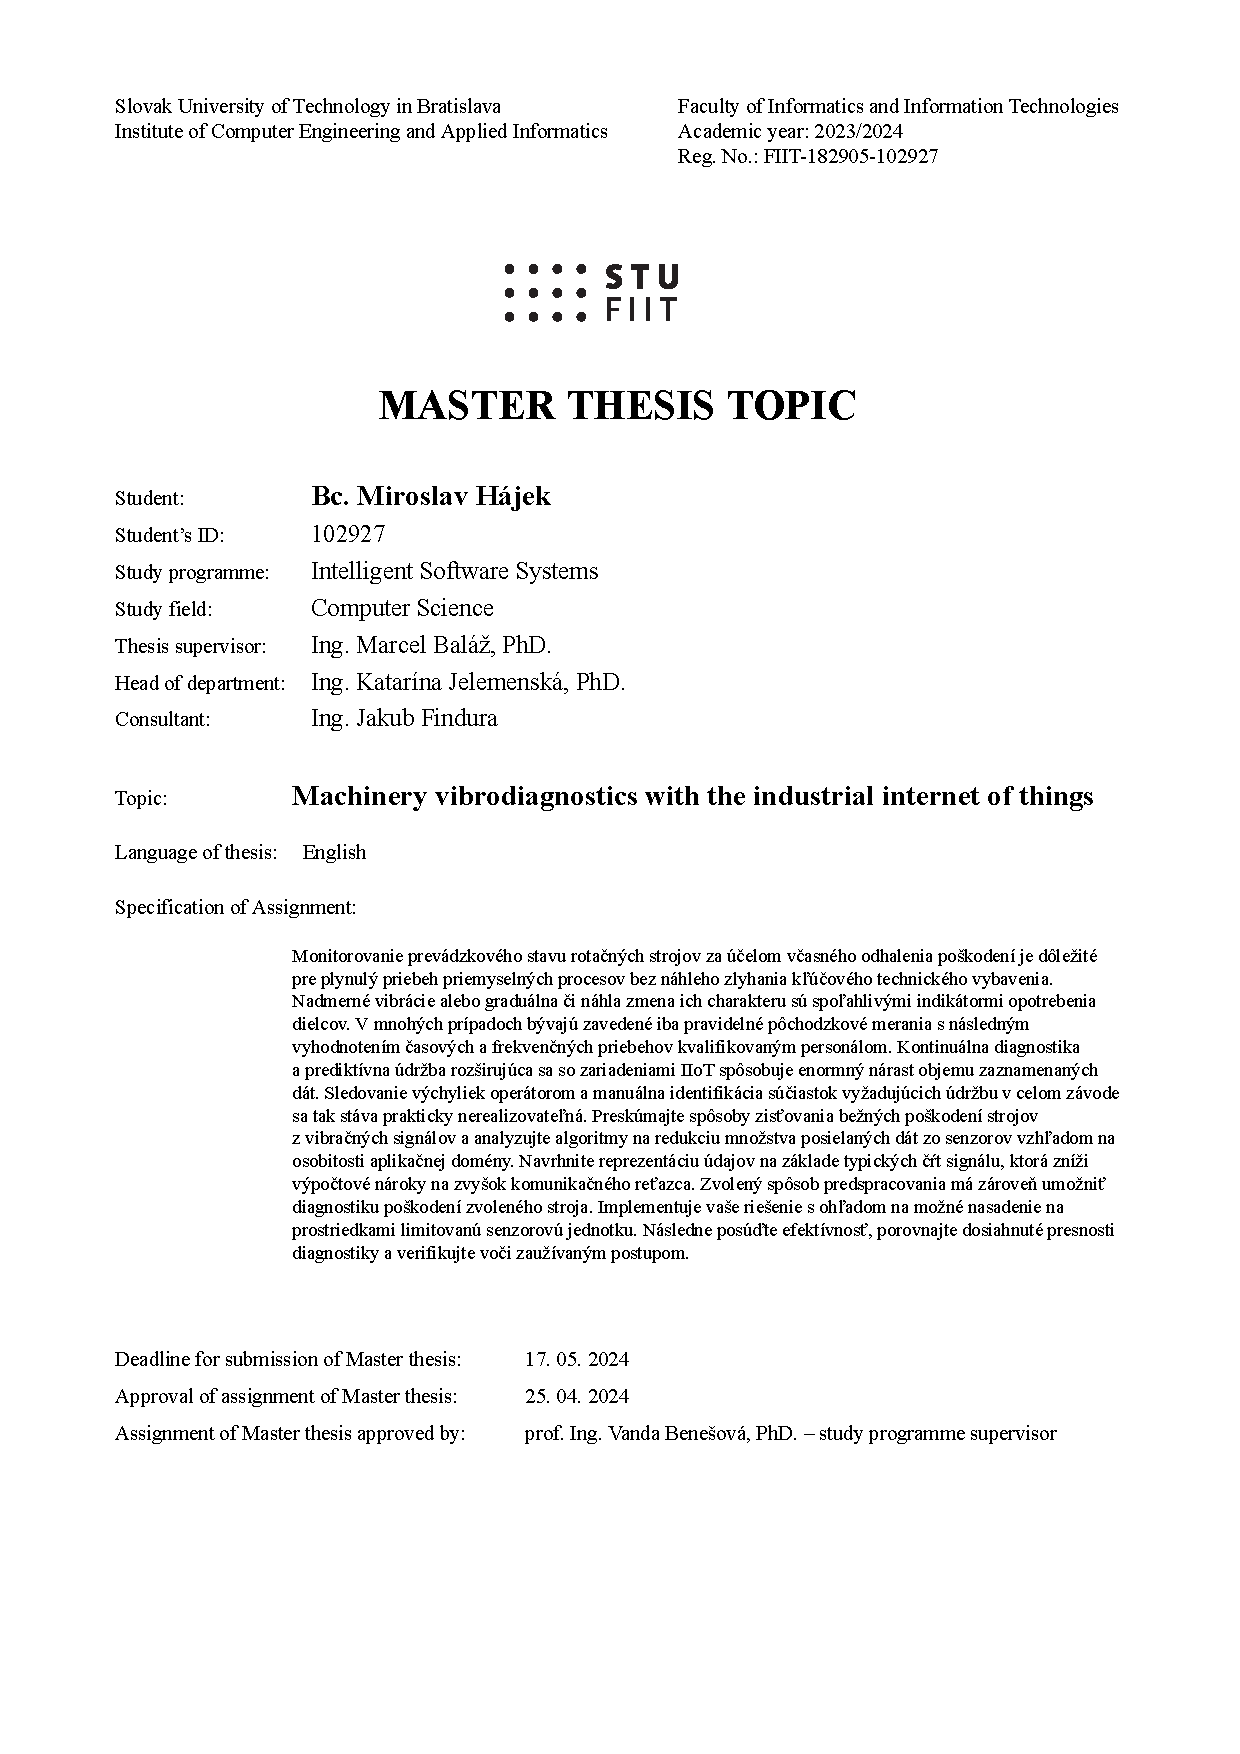
\includepdf[pages=-, scale=1]{chapters/topic}
\emptypage

% Thesis assignment
\thispagestyle{empty}

\includepdf[pages=-, scale=1]{chapters/assignment}
\emptypage
\emptypage

% Declaration of Honour
 % Declation of Honour
\thispagestyle{empty}
\vspace*{\fill}
\section*{Declation of Honour}

I hereby declare on my honour that I wrote this thesis independently under supervision of Dr. Marcel Baláž, after consultations and with use of cited literature.

\vspace{3\medskipamount}\noindent
\SignPlace \SignDateEN \hspace*{\fill} \signaturespace{5cm}{\Author} 

\emptypage

% Acknowledgments
% Poďakovanie
\thispagestyle{empty}
\vspace*{\fill}
\section*{Acknowledgement}

\vspace{3cm}
\emptypage

% Annotations
\thispagestyle{empty}
\section*{Annotation}
\UniversityEN \\
\uppercase{\FacultyEN}
\vspace{-8pt}
{\setlength{\mathindent}{0cm}
\begin{align*}
&\text{Degree course:} && \text{\StudyProgrammeEN} \\
&\text{Author:} && \text{\Author} \\
&\text{\ThesisEN:} && \text{\TitleEN} \\
&\text{Supervisor:} && \text{\SupervisorEN} \\
&\text{\DateEN}
\end{align*}}

\emptypage 

\thispagestyle{empty}
\section*{Anotácia}
\University \\
\uppercase{\Faculty}
\vspace{-8pt}
{\setlength{\mathindent}{0cm}
\begin{align*}
&\text{Študijný program:} && \text{\StudyProgramme} \\
&\text{Autor:} && \text{\Author} \\
&\text{\Thesis:} && \text{\Title} \\
&\text{Vedúci diplomovej práce:} && \text{\Supervisor} \\
&\text{\Date}
\end{align*}}

\emptypage

% Contents
\pagestyle{empty}
\tableofcontents{}
\listoffigures
\listoftables
\listofmyequations

% {\let\clearpage\relax }
\printnomenclature
\emptypage
\emptypage

\pagestyle{fancy}
% Chapters
\pagenumbering{arabic}

\chapter{Introduction}
Manufacturing is experiencing a shift in the traditional practices of asset operational status evaluation and utilization. The rise of Industry 4.0 means greater automation and robotization of the production halls to achieve optimal usage of available resources. The secondary aspect in the enterprises' endeavor, however not less important, is to keep track of the equipment wear and tear. The corrective action be it repair or replacement should be taken on time in response to the key indicators. 

The goal is to preserve required safety and production efficiency when extending the useful life of machine moving parts. In the factories and logistics where this sort of equipment is vital, there is a rising interest in the ability to monitor in real-time the health of the machines and to proactively diagnose the fault to repair it without adding unnecessary costs. 

Vibrations are the most nonintrusive way with which such faults can be sensed. The experts use it to distinguish faulty states and to identify the malfunction's root cause. In critical circumstances such as in the case of the large turbines in the power plants, the precautions leading to regular machinery check-ups are already in place. To reach wider acceptance and spread, the monitoring solution has to be sufficiently independent, reliable, and as self-sufficient as the model design allows it to be.

The main issue to consider in large-scale machinery monitoring using vibrations are lots of uninformative streams of samples not directly useful for the production line operator. The dashboard must aggregate these flows into trend variables with severity levels categorized based on industrial standards. The majority of signals are viewed once at the maximum therefore to store or even transmit them from the edge device in its entirety would be wasteful. The complex overview of the mechanical equipment status is attainable only when agent devices and sensors are cheap enough with a long lifespan on battery power and preferably remain physically small to reduce the additional clutter.

Attempted machine and deep learning approaches have the crucial impediment that the construction of every single machine is unique to some extent because of tolerances and variable load. The model must be trained specifically for the target environment to achieve the ideal performance. In addition, the failures are relatively rare events occurring usually in the span of multiple months. In these circumstances, it is hard to obtain a large enough sample of fault events quickly. Novelty detection is a technique that can be applied in this case.

The thesis is organized in the following manner. In the first chapter of analysis in section 1 we explore the mechanical maintenance approaches and industry standards on common fault identification. Then section 2 is all about measuring vibrations and transforming them into features meaningful in automatic fault pattern recognition. In section 3 we delve into modes of diagnosis based on reduced relevant indicators. Section 4 deals with evaluation datasets used to determine computational requirements
on IIoT infrastructure. Chapter 2 defines data format and proposes processing steps to diagnose the imminent failure and different fault types. The approach taken is evaluated and validated in Chapter 6. 
  

\chapter{Problem analysis}


\section{Condition monitoring}

What are predicted variables - result of diagnoses
\begin{itemize}
\item - Presence of the Fault
\item Type of fault present (different characteristics - e.g. frequency content)
\item Remaining Useful Life (time until failure) - machines of the same type and different degradation curves
\end{itemize}

\textbf{Remainig useful life models} (RUL) - is the expected life or usage time remaining before the machine requires repair or replacement.
\url{https://www.mathworks.com/help/predmaint/ug/rul-estimation-using-rul-estimator-models.html}
\begin{itemize}
\item Similarity - run to failure history of similiar machines in database
\item Degradation - known failure threshold (warning, alert threshold)
\item Survival  - life-span of components and correlated variables
\end{itemize}


\cite{jung_vibration_2017}
\begin{itemize}
\item Indirect Measurement: indirect and approximate measurement over the vibration phenomenon of the target equipment.
\item Noisy and Unaligned Observations: well aligned / may contain huge amount of noise.
\item Variance on Initial Status: initial status of the target equipment different from each other.
\item Diversity on Lifetime model: the usage and lifetime model -  number of unknown and external factors.
\end{itemize}

\subsection{Maintenance strategies}
Difference between fault (degrating performace of the machine - higher friction and power consumption) and failure (machine is unusable). \cite{mohanty_machinery_2015} (picture)
\begin{itemize}
\item Reactive - run equipment until failure occurs - low stakes operation. Failure can have negative economic impact or can damage adjacent parts
\item Preventive - predetermined schedule when assets are diagnosed and repairs are made. Crutial to set appropiate maintanance interval. Good parts are replaced before they are completely worn out, preventing critical failure, but creating unneccesary waste. Sometimes faults are not detected soon enough.
\item Predictive - model of expected lifetime, warns about unexpected faults before they become too serious and before affecting the machine.
\end{itemize}

Wear process curve \cite{mohanty_machinery_2015} Bath tub curve (page 10)
\begin{itemize}
	\item Initial - large roughness
	\item Normal - contact area fomred
	\item Severe - high friction
\end{itemize}

Rotordynamics (chapter 4) (p. 29)  - p.97 - Fault types, p.127 - faults in electric motors

In order to understand, and correctly diagnose the vibratory characteristics of rotating machinery, it is essential for the machinery diagnostician to understand the physics of dynamic motion. This includes the influence of stiffness and damping on the frequency of an oscillating mass — as well as the interrelationship between frequency, displacement, velocity, and acceleration of a body in motion. \cite{eisenmann_machinery_1997}
\begin{itemize}
\item Forced Vibration Mechanism
	\begin{itemize}
	\item Mass Unbalance
	\item Misalignment
	\item 	Shaft Bow
	\item Gyroscopic
	\item Gear Contact
	\item Rotor Rubs
	\item Electrical Excitations
	\item External Excitations
	\end{itemize}
\item Free Vibration Mechanism
	\begin{itemize}
	\item Oil Whirl
	\item Oil or Steam Whip
	\item  Internal Friction
	\item Rotor Resonance
	\item Structural Resonances
	\item Acoustic Resonances
	\item Aerodynamic Excitations
	\item Hydrodynamic Excitations
	\end{itemize}
\end{itemize}

\subsection{Vibration fault types}
There are a few methods of machinery fault identification in vibrational signals based on domain expertise. Data points can be viewed in the time domain and frequency domain. Either as individual stationary profiles obtained during the short duration in the time of measurement, or multiple spaced-out observations with the intent to highlight the long-term trend, e.g. shown in a waterfall plot \cite{ziaran_technicka_2013}. The descriptor variable can be any meaningful statistical quantity, e.g. peak-to-peak, RMS, crest factor, kurtosis, which can be applied to recorded samples or frequency bands.

Mechanical faults manifest themselves in the vibration signal at various frequencies. In the low-frequency range (up to 1 kHz) shaft's unbalance, misalignment, bend, crack, and mechanical looseness is present. High frequencies (up to 16 kHz or more) contain bearings faults and gear faults.

Under fault-free circumstances, shaft speed appears as the strongest frequency component. In case of shaft and gear imbalance or damage, synchronous multiples of shaft frequency (harmonics) are amplified. When rub, bad drive belts and chains, or looseness is occurring in the machine then sub-synchronous harmonics or even non-synchronous frequencies appear \cite{mohanty_machinery_2015}.  Therefore it is useful to rescale the horizontal axis to RPM or orders of rotational speed. Complementary methods of fault symptom identification are phase and orbital analysis \cite{scheffer_practical_2004}.

\begin{itemize}
\item Bearing faults - vibration on each rotation of rolling elements, CFC (characteric fault frequencies with impulse
\item Rotor bar faults - current will not flow - forces diffrent on both sides of rotor
\item Eccentricity Faults - uneven air gap between stator rotor
\item Misalignment - parralel / angular
\item Cavitation - pumps
\item Gearbox fault -broken teeth
\end{itemize}
measuring vibration with current, thermal, flux is improvement, +acoustic elminited (detect similiar faults)
vibration is better alone, then other methods alone (80 vs. <60%)
 \cite{goel_methodology_2022}

\subsection{Technical standards}
The maintenance procedure usually involves data acquisition cards inside handheld devices with accelerometer sensor probes then mounted firmly to the machine frame by either screwing in, magnets or wax \cite{ziaran_technicka_2013}. The probe placement in axial and perpendicular radial directions is standardized in ISO 20816. The severity of vibrations is mostly assessed in units of velocity ($mm/s$), but acceleration ($m/s^2$) and displacement ($\mu m$) are also used. Based on the observed vibration intensity and one of the four classes of machines (I, II, III, IV) by output power and size, zones (A, B, C, D) for accepted levels are proposed. It is customary to establish operational limits in the form of alarms and trips \cite{iso_20816}.

Standard ISO 13373 categorizes three types of vibration monitoring systems: permanent, semi-permanent, and mobile. More importantly, a structured diagnostic approach is developed here complete with recommendations for formalizing diagnostic techniques \cite{iso_13373}. The next step is the signal analysis with the use of proper units and transformations is the subject of the ISO 18431 \cite{iso_18431}.

ISO-10816 Vibration Severity Chart
Typical faults produce unusual low-frequency vibrations (10 to 1000 Hz).
Imbalances, misalignments and looseness are recorded at frequencies up to 300 Hz.

\paragraph{Sensor placement}

\section{Feature engineering}
\subsection{Feature extraction}
Statistical features in Time-domain (and correlation to blade wear) \cite{zhuo_research_2022} \cite{zheng_feature_2018}
\begin{itemize}
	\item 	Root mean square (0.98)
	\item Mean (0.17)
	\item Amplitude (0.81)
	\item Kurtosis (0.042)
	\item Peak to peak (0.463)
	\item Signal strength (0.119)
	\item Standard deviation (0.908)
	\item Peak value (0.488)
	\item Shape factor (0.007)
	\item Skewness (0.118)
	\item Avearge signal level (0.46)
	\item Crest factor (0.056, spikeness of the signal - rms/amplitude)
\end{itemize}
Selection according to high correlation (graph: sawn-trough section vs feature)
Features in time domain with high correlaction: RMS, Standard deviation, Amplitude

Statistical features in Frequency domain (PSD analysis) r >= 0.8 db3 analysis
\begin{itemize}
	\item 	Root mean square (0.402)
	\item Mean (0.497)
	\item Peak frequency (0.670)
	\item Kurtosis (0.852)
	\item Peak to peak (0.076)
	\item Standard deviation (0.799)
	\item Peak value (0.787)
	\item Shape factor (0.851)
	\item Skewness (0.819)
	\item Frequency centroid (0.775)
\end{itemize}
skewness (PSD\_S), kurtosis (PSD\_k), and shape factor (PSD\_Sf),
centroid frequency (FFT\_fc), wavelet packet energy entropy (WPD\_EP) = 0.85
- The WPD energy E8, E10, and E12
- Energy ratios P8 and P13 of frequency bands 8 and 13

Spectral features \cite{peeters_large_2004} - 1. Spectral shape description
\begin{itemize}
\item Coherence function - correlation between two signals PSD
\item  Spectral centroid - barycenter of the spectrum (weighted mean of the frequencies present in the signal, with their magnitudes as the weights)
\item Spectral spread
\item Spectral skewness
\item Spectral kurtosis
\item Spectral slope - comupted with linear regression - amount of decresing of the spectral amplitude
\item Spectral roll-off - 95\% of the signal energy is contained below this frequency
\item 2. Temporal variation of spectrum - spectral flux - correlation of normalized cross-correlation between two succesive amplitude spectra
\end{itemize}

Harmonic features
\begin{itemize}
\item Fundamental frequency  - Maximu likelihood algorithm
\item Noisiness - ratio - energy of noise to the total energy
\item Inharmonicity - energy weighted difference of the spectral components from the multiple of fundamental frequency
\item Harmonic Spectral Deviation - deviation of amplite harmonics peaks from global spectral envelope
\end{itemize}

\textbf{Harmonic peak feature} - \cite{jung_vibration_2017}- group of pairs of significant peaks’ value and frequency in PSD. Harmonic peak distance Dij

\begin{itemize}
\item Standardization - Min-max scaler, Standard scaler (clustering - feature have different scales)
\item Transformation - Log transformation, Box-Cox
\end{itemize}

major drawbacks of PSD
\begin{itemize}
	\item PSD is a highdimensional feature (i.e., 1024 dimensions in our case) that often generates singular matrix = regression algorithms.
	\item PSD feature is unreliable due to a large random fluctuation in their amplitudes over frequency due to measurement noise inherent in MEMS sensor.
\end{itemize}


\subsubsection{Signal denoising and filtering}
Blind source separation, PCA, ICA
vibration analysis tools:
\begin{itemize}
\item ICA (independent component analysis),
\item TFA (time-frequency analysis),
\item ED (energy distribution) and
\item CD (change detection)
\end{itemize}

\subsubsection{Time-frequency features}
The PSD is the overall expectation of the AE signal. It needs to be calculated by estimation methods. The estimation of the power spectrum is realized by Welch method (cite)

Time Synchronous Averaging of Real FFT
vs. FastCWT - Synchrosqueezing

\subsubsection{Harmonics identification}
Cepstrum + Harmonic Product Spectrum + Peak identification


\subsection{Feature selection}
Feature importance ranking of Numeric features - Filtering
\begin{itemize}
\item High correlation with predictor - band saw blade width of flank face --- to signal statistics
\item Low correlation (Decorrelation) among predictors themselves - if they are correlated they produce same response
\item ANOVA with F-Test - Variance of the feature - high variance - is high response
\item Linearly dependent features are a waste of space and computation power because the information could have been encoded in much fewer features. \cite{zheng_feature_2018} - solve by PCA
\end{itemize}

Vibration levels are dependent on the type of work (load) of the machine (cite)
\begin{itemize}
\item \textbf{Sawing process database}: it contains basic information such as sawing machine tools model, band saw blade model, sawing parameters, and the material and size of the workpiece to match the relevant online monitoring model.
\item \textbf{Online monitoring model database}: it stores online monitoring models of band saw blade wear based on different sawing processes.
\end{itemize}

\section{Diagnostics techniques}
\url{https://scikit-learn.org/stable/modules/outlier_detection.html#outlier-detection}
\subsection{Novelty detection}
\textbf{Fault or no fault} - anomaly detection solutions - unsupervised \cite{torres_automatic_2022}. mean shift clustering algorithm
\begin{itemize}
\item Robust Covariance  (Mahalanobis distance)
\item One-class SVM with non-linear kernel (RBF) - classifying new data as similar or different to the training set
\item Local outlier factor - local density deviation of a given data point with respect to its neighbours
\item Isolation forest
\end{itemize}

\textbf{Types of faults - clustering}
\begin{itemize}
\item BIRCH
\item DBSCAN - density based params:
	minPts (the minimum number of data points that need to be clustered together for an area to be considered high-density)
	eps (the distance used to determine if a data point is in the same area as other data points).
\item OPTICS - better DBSCAN -  clusters in data of varying density
\end{itemize}

\subsection{Label propagation in semi-supervised learning}

Transductive Support vector machine(TSVM),
Label Propagation Algorithm(LPA)

\section{IoT in Industry 4.0}
	Wireless protocols limitation: IEEE 802.11, IEEE 802.15.4e, OpenThread
	Power consumption
	Devices and sensors

	The Fig. 1 shows a generalist architecture supported in the context of Industry 4.0, fault detection systems in electrical machines based on vibration analysis  The Operational Technology (OT) and Information Technology (IT) parts were aligned to design an Industrial Control System (ICS) in the laboratory, for acquiring, controlling and monitoring the operating status of rotating machines, producing reports, automatic alerts and recommending actions to take as a prescriptive maintenance system. \cite{torres_automatic_2022}


\chapter{Design}

\section{Research questions}
\begin{enumerate}
\item \emph{Which time-frequency features can be extracted from vibrational signals to provide an accurate record of machinery faults?}
\item \emph{What are the savings in transmission bandwidth when chosen signal features are used in comparison to raw sampled measurement or lossless compression techniques?}
\item \emph{How can the machinery faults be continuously identified based on collected events?}
\end{enumerate}

\section{Infrastructure}
 \begin{itemize}
\item \textbf{Input:} Samples from acceleration in 3-axis, RPM, Noise background
\item \textbf{Output is either:} machine overall status, type of fault, remaining useful life
\item \textbf{Output for domain expert}: Annotation interface, Control chart of trend features, Power frequency spectrum, Waterfall plot
 \end{itemize}

\begin{enumerate}
\item MEMS accelerometers are placed on at least two distinict measurement points in two perpendicular axis and one sensor in base for denoising. Rotational speed is captured at the same time too.
\item Sensors are triggered in regular intervals (every 15 minutes) to collect sample recording from the band saw. Configurable parameters set based on experiments: sampling frequency, dynamic range, window type (Hamming) and size (based on resolution), PSD estimation method (Welch)
\item \textbf{Features} are computed and compared to recent measurements. If there is an statistically significant change the whole summary is send, otherwise keepalive notification is send.
\item Possible local communication between sensors to pre-compute clustering information
\item Database stores history of measurements
\item \textbf{Diagnosis panel runs clustering} with introduction of annotations to notify the operator about observed fault and imminent failure of the machine.
\end{enumerate}

Nároky na hardvér ako výstup analýzy - koprocesor (výpočet) - inštruckčná sada, real time odozva, ramka pri oknách



\chapter{Implementation} \label{chapter:implementation} 

\section{Data analysis}
% Jupyter notebook - TSFEL, numpy, pandas (data handling),  scipy (signal processing and stats),   | sklearn, imblearn | matplotlib


\section{Firmware}
% In C, ESP-IDF SDK and FreeRTOS tasks
% Found driver online
% Problems with timing - binary write (osciloscope pictures)
% tool for convert bin2csv


\begin{figure}[h]
    \centering
    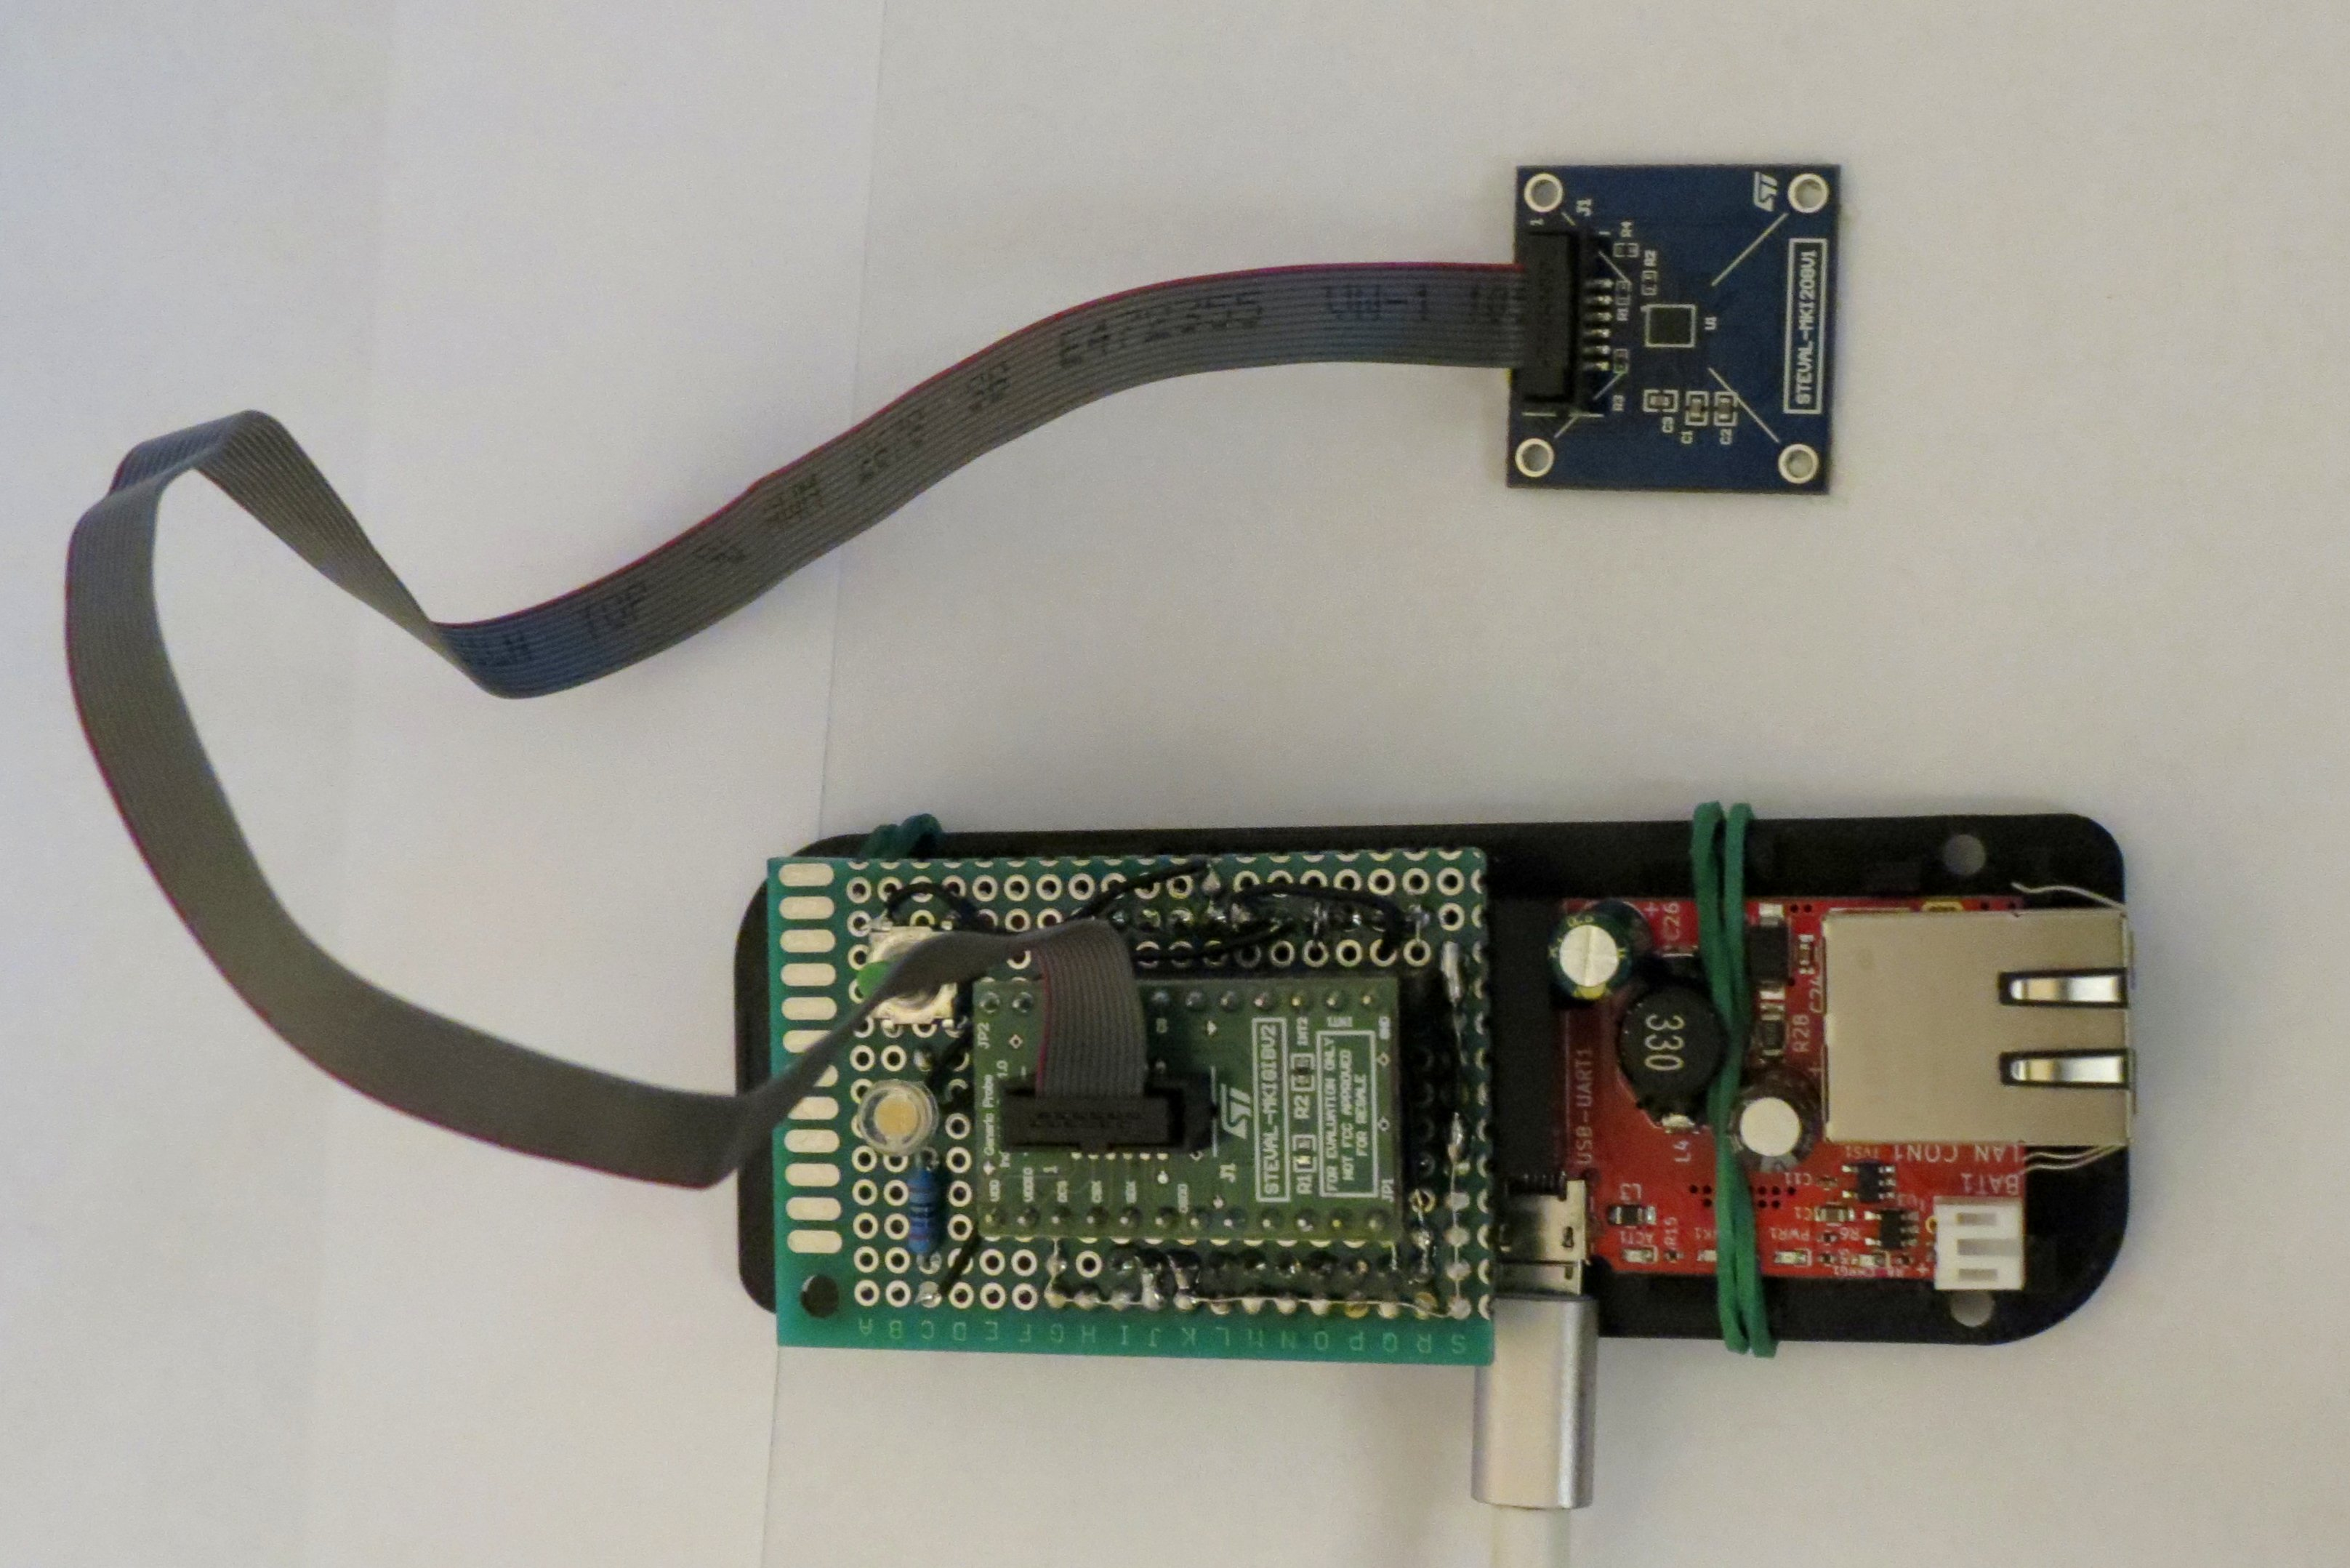
\includegraphics[width=0.5\textwidth]{assets/design/sensor/data-logger.jpg}
    \caption{Accelerometer Data Logger}
\end{figure}




\chapter{Evaluation} \label{chapter:evaluation}
The verification of proposed solutions for machinery fault diagnostics is focused on two complementary activities, these are vibration measurement and defect identification. The accuracy of supervised learning using the k-nearest neighbour classifier is determined by the MaFaulDa dataset under various experiments. Data logger recording is compared to the known reference, and the collected Pump dataset is analyzed.

\section{MaFaulDa in k-nearest neighbors}
The four outlined experiments on MaFaulDa involve testing sets of features with very few members to see the effects in predictions when reducing the information content about machine status to the minimum. First, the attributes are left in the complete count after extraction. Then, all of their combinations are enumerated, and the resulting accuracy distribution is matched against accuracy after feature selection with similarity metrics. 

\subsection{Complete feature sets}
The two full sets of features include ten extracted from time-domain and eleven from frequency-domain of the vibrations. The feature spaces can incorrectly interchange different fault labels and better separate out some groups than the others. 

\begin{figure}[h]
    \centering
    \begin{subfigure}[b]{0.49\textwidth}
        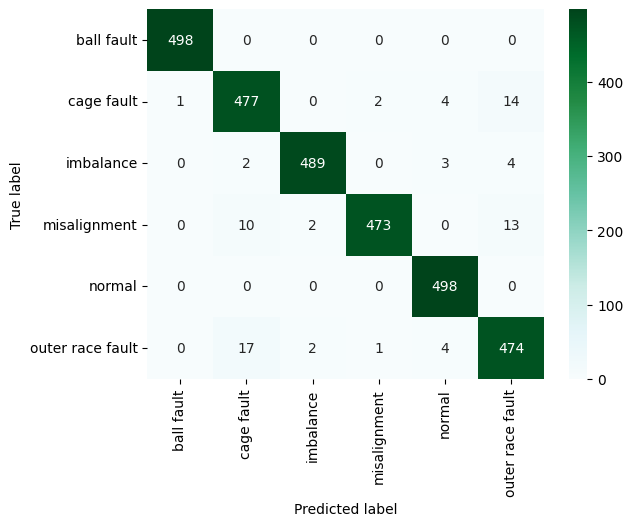
\includegraphics[width=\textwidth]{assets/results/all-features/TD-confusion-matrix.png}
        \caption{Time-domain features}
    \end{subfigure}
    \hfill
    \begin{subfigure}[b]{0.49\textwidth}
        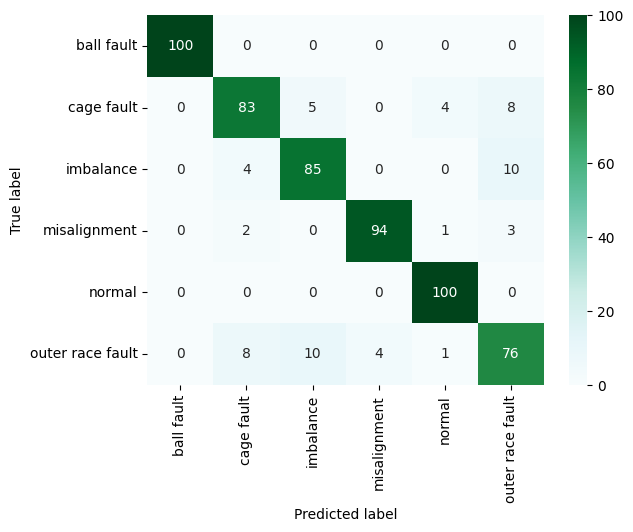
\includegraphics[width=\textwidth]{assets/results/all-features/FD-confusion-matrix.png}
        \caption{Frequency-domain features}
    \end{subfigure}
    \caption{Confusion matrix for complete sets of features}
    \label{fig:evaluation:all-features-confusion-matrix}
\end{figure}

The inner bearing observations are selected to train the k-NN with five neighbours and Euclidean distance metric. The attributes are normalized beforehand, rows are oversampled to a majority label, and data is split into training and testing sets with an 80:20 proportion. The 598 observation of validation data determines the confusion matrix (Fig.~\ref{fig:evaluation:all-features-confusion-matrix}). 

The label ``normal'' is not falsely attributed to other classes in either feature set, but other classes can get assigned to be ``normal''. Most mistakes happen while predicting outer race fault, which is confused with cage fault, imbalance, and less frequency with misalignment. The shaft imbalance is used for simulating bearing faults, which is a natural reason for this high error rate.

\begin{figure}[h]
    \centering
    \begin{subfigure}[b]{0.48\textwidth}
        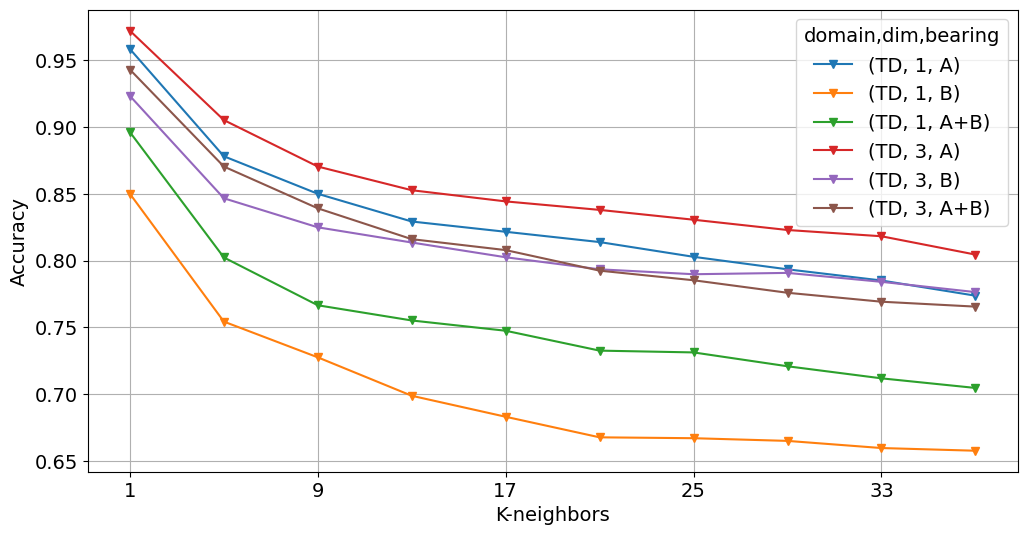
\includegraphics[width=\textwidth]{assets/results/all-features/TD.png}
        \caption{Time-domain features}
    \end{subfigure}
    \hfill
    \begin{subfigure}[b]{0.48\textwidth}
        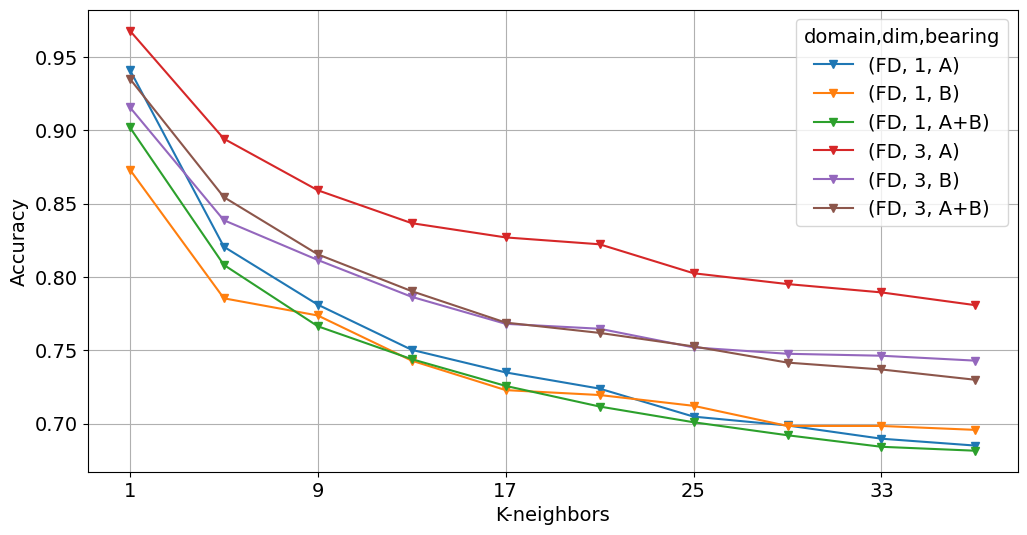
\includegraphics[width=\textwidth]{assets/results/all-features/FD.png}
        \caption{Frequency-domain features}
    \end{subfigure}
    \hfill
    \begin{subfigure}[b]{0.48\textwidth}
        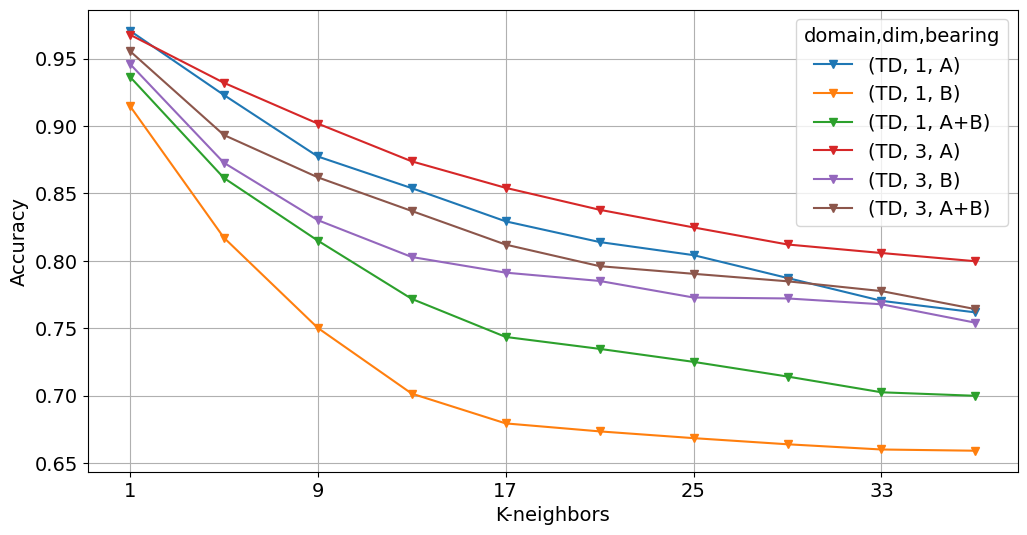
\includegraphics[width=\textwidth]{assets/results/all-features/TD-severity.png}
        \caption{Time-domain features (severity)}
    \end{subfigure}
    \hfill
    \begin{subfigure}[b]{0.48\textwidth}
        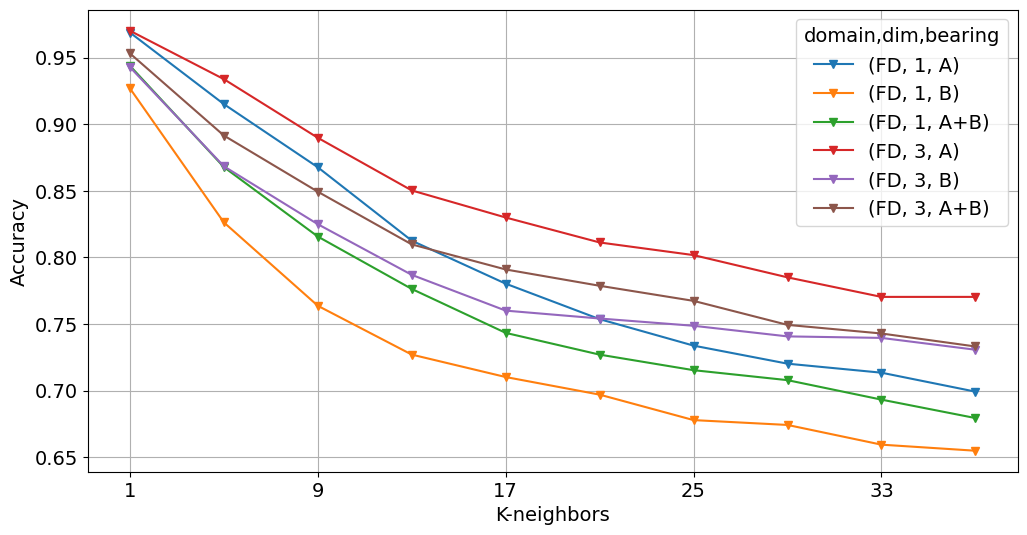
\includegraphics[width=\textwidth]{assets/results/all-features/FD-severity.png}
        \caption{Frequency-domain features (severity)}
    \end{subfigure} 
    \caption{Accuracy on complete feature sets depending on the k-value}
    \label{fig:evaluation:complete-set-k-value}
\end{figure}

The increasing number of neighbours used for classification in 5-fold cross-validated k-NN shows a substantial decrease in accuracy on validation sets (Fig.~\ref{fig:evaluation:complete-set-k-value}). The most prominent drop in performance of around 10\% occurs at the beginning until the k-value of nine, and then the accuracy curves slowly plateau.

Under every circumstance, the magnitude of the triaxial feature vector reaches better accuracy than those from only the axis of motion for the same source domain and bearing. The model for inner bearing A is more accurate than outer bearing B. The TD set is generally better in predictions than the FD set for the equivalent k-value. The relabeled dataset for high severity has a steeper decrease in accuracy for the same value of neighbours.


\subsection{Feature subset combinations}
The complete sets of predictors are even greatly shrunken to representation that could be presented in 3D plot or in perpendicular cross sections. These trend variables could be used in distingushing faults the same way as rms amplitude indicates their presence. Each possible combinations of pairs, triplets, and quadruplets constructs a separate k-NN model on which prediction accuracy is evaluated. 

\begin{figure}[h]
    \centering
    \begin{subfigure}[b]{0.48\textwidth}
        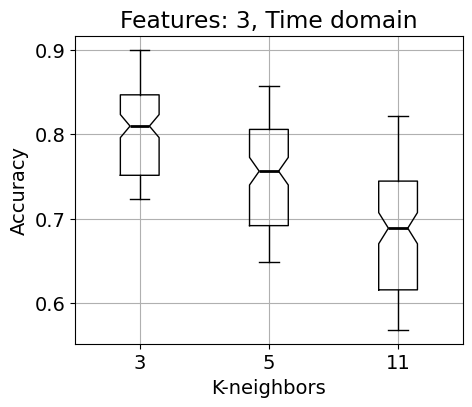
\includegraphics[width=\textwidth]{assets/results/feature-combinations/TD-3-A-False-False-F3.png}
        \caption{Three time-domain features}
    \end{subfigure}
    \hfill
    \begin{subfigure}[b]{0.48\textwidth}
        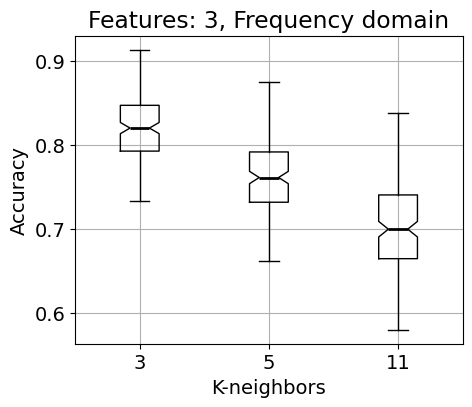
\includegraphics[width=\textwidth]{assets/results/feature-combinations/FD-3-A-False-False-F3.png}
        \caption{Three frequency-domain features}
    \end{subfigure}
    \hfill
    \begin{subfigure}[b]{0.48\textwidth}
        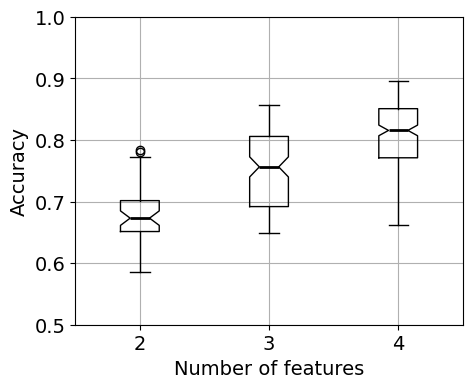
\includegraphics[width=\textwidth]{assets/results/feature-combinations/TD-3-A-False-False-K5.png}
        \caption{Five neighbours in time domain}
    \end{subfigure}
    \hfill
    \begin{subfigure}[b]{0.48\textwidth}
        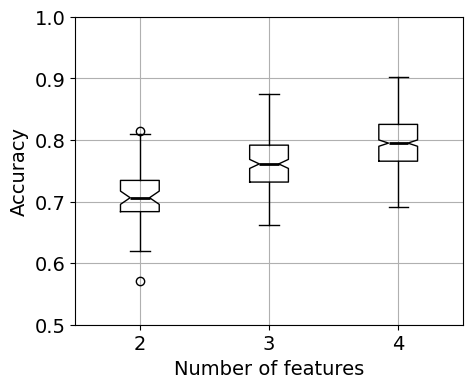
\includegraphics[width=\textwidth]{assets/results/feature-combinations/FD-3-A-False-False-K5.png}
        \caption{Five neighbours in frequency domain}
    \end{subfigure}
    \caption{Model accuracy distribution for bearing A and three axis features}
    \label{fig:evaluation:model-accuracy}
\end{figure}

\begin{figure}[h]
    \centering
    \begin{subfigure}[b]{0.48\textwidth}
        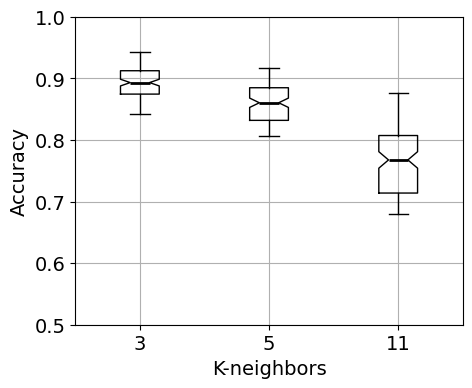
\includegraphics[width=\textwidth]{assets/results/feature-combinations/TD-3-A-True-False-F3.png}
        \caption{Three time-domain features}
    \end{subfigure}
    \hfill
    \begin{subfigure}[b]{0.48\textwidth}
        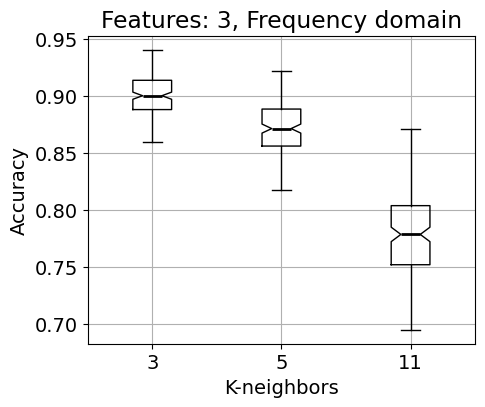
\includegraphics[width=\textwidth]{assets/results/feature-combinations/FD-3-A-True-False-F3.png}
        \caption{Three frequency-domain features}
    \end{subfigure}
    \hfill
    \begin{subfigure}[b]{0.48\textwidth}
        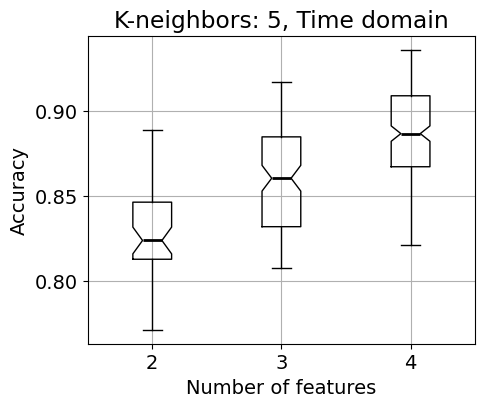
\includegraphics[width=\textwidth]{assets/results/feature-combinations/TD-3-A-True-False-K5.png}
        \caption{Five neighbours in time domain}
    \end{subfigure}
    \hfill
    \begin{subfigure}[b]{0.48\textwidth}
        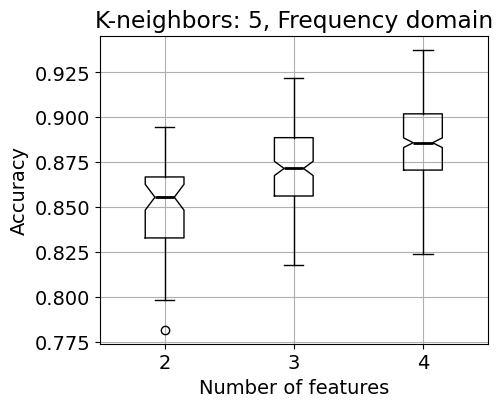
\includegraphics[width=\textwidth]{assets/results/feature-combinations/FD-3-A-True-False-K5.png}
        \caption{Five neighbours in frequency domain}
    \end{subfigure}
    \caption{Model accuracy distribution from bearing A and three axis features after relabeling for high severity faults}
    \label{fig:evaluation:model-accuracy-severity}
\end{figure}

The distribution of model accuracies is documented on features in both domains coined from three dimensions on bearing A with original and high-severity defect labels. The boxplots display the relation of the k-value to accuracy when three features are chosen, and the relation of a number of features to accuracy with five neighbours(Fig.~\ref{fig:evaluation:model-accuracy-severity} and \ref{fig:evaluation:model-accuracy-severity}).

The decrease in accuracy with additional neighbours is apparent and similar to the trend in complete sets of features. We are interested in maximum accuracy in the distribution because that is the optimal model feature selection method to try to approach. Its reduction is more noticeable between three and five features 3 - 5\%, and almost the same amount between five and eleven neighbours. 

The complete sets reach better accuracy than subsets when the number of features is at most three and simultaneously the number of neighbours is five or less. For more triaxial features and more neighbours, the complete set is only about 2\% percent worse at the most than subsets because the curse of dimensionality is not so substantial for ten dimensions.

The spread in model accuracies in the interquartile range is from 5 to 10 \%, and measured between whiskers is at a maximum of 25\%. The standard deviation is about 7\%. Overall, the time-domain features are better than frequency-domain features for these specific feature spaces.

The number of features has a direct proportionality effect on the optimal model accuracy. An increase from two to three features has more weight than allowing a fourth attribute. The contributions of adding features are around 6\% and 3\%, and the relabeled dataset has an increase of 3\% and 2\%. The absolute accuracies are consecutively for 2, 3, and 4 features when k is equal to 5: 78.31\%, 85.67\%, and 89.55\% for the time domain and 81.52\%, 87.52\%, 90.26\% in the frequency domain.


\subsection{Feature selection techniques}
The predictors chosen with supervised selection strategies are compared in accuracy and location within the accuracy distribution of exhaustive combinations of same-sized sets and the performance of its source superset. The metrics for bivariate feature selection are correlation, F statistic, mutual information, and their ensemble by the rank product. The PCA of the complete feature set that retains the same number of features and selection methods serves as a benchmark to tell whether the linear combination or subset gets better performance on the MaFaulDa.

\begin{table}[h]
\centering
\begin{adjustbox}{width=\textwidth}
\begin{tabular}{|l|rr|rr|r|l|}
\hline
\multirow{2}{*}{\textbf{Feature set}} & \multicolumn{2}{l|}{\textbf{Accuracy}}                                   & \multicolumn{2}{l|}{\textbf{Percentile}}                 & \multicolumn{1}{l|}{\multirow{2}{*}{\textbf{Domain}}} & \multirow{2}{*}{\textbf{Best features}} \\ \cline{2-5}
                                      & \multicolumn{1}{l|}{\textbf{Train}} & \multicolumn{1}{l|}{\textbf{Test}} & \multicolumn{1}{l|}{\textbf{Train}} & \multicolumn{1}{l|}{\textbf{Test}} & \multicolumn{1}{l|}{}                               &                                         \\ \hline
All features                          & \multicolumn{1}{r|}{96.03}          & 92.80                              & \multicolumn{1}{r|}{100.00}         & 100.00                             & TD                                                   &                                         \\ \hline
PCA PC                                & \multicolumn{1}{r|}{91.20}          & 84.67                              & \multicolumn{1}{r|}{95.00}          & 93.33                              & TD                                                   &                                         \\ \hline
Best features                         & \multicolumn{1}{r|}{91.93}          & 85.47                              & \multicolumn{1}{r|}{100.00}         & 99.17                              & TD                                                   & zerocross, pp, skewness                 \\ \hline
Rank product                          & \multicolumn{1}{r|}{91.21}          & 85.04                              & \multicolumn{1}{r|}{95.83}          & 97.50                              & TD                                                   & zerocross, shape, rms                   \\ \hline
Correlation                           & \multicolumn{1}{r|}{91.21}          & 85.04                              & \multicolumn{1}{r|}{95.83}          & 97.50                              & TD                                                   & shape, zerocross, rms                   \\ \hline
F statistic                           & \multicolumn{1}{r|}{90.59}          & 84.07                              & \multicolumn{1}{r|}{91.67}          & 90.00                              & TD                                                   & rms, pp, zerocross                      \\ \hline
Mutual information                    & \multicolumn{1}{r|}{88.24}          & 80.62                              & \multicolumn{1}{r|}{75.83}          & 76.67                              & TD                                                   & zerocross, shape, crest                 \\ \hline
All features                          & \multicolumn{1}{r|}{93.67}          & 88.45                              & \multicolumn{1}{r|}{100.00}         & 100.00                             & FD                                                  &                                         \\ \hline
PCA PC                                & \multicolumn{1}{r|}{86.76}          & 78.51                              & \multicolumn{1}{r|}{64.85}          & 70.91                              & FD                                                   &                                         \\ \hline
Best features                         & \multicolumn{1}{r|}{92.86}          & 87.52                              & \multicolumn{1}{r|}{100.00}         & 100.00                             & FD                                                   & centroid, roll\_off, entropy            \\ \hline
Rank product                          & \multicolumn{1}{r|}{85.79}          & 77.18                              & \multicolumn{1}{r|}{51.52}          & 57.58                              & FD                                                   & roll\_off, flux, skewness               \\ \hline
Correlation                           & \multicolumn{1}{r|}{85.79}          & 77.18                              & \multicolumn{1}{r|}{51.52}          & 57.58                              & FD                                                   & roll\_off, skewness, flux               \\ \hline
F statistic                           & \multicolumn{1}{r|}{85.79}          & 77.18                              & \multicolumn{1}{r|}{51.52}          & 57.58                              & FD                                                   & roll\_off, flux, skewness               \\ \hline
Mutual information                    & \multicolumn{1}{r|}{90.73}          & 83.60                              & \multicolumn{1}{r|}{94.55}          & 94.55                              & FD                                                   & roll\_off, entropy, noisiness           \\ \hline
\end{tabular}
\end{adjustbox}
\caption{Feature selection method accuracy and percentile within accuracy distribution of all three member subsets. (bearing = A, dimension = 3, k=5)}
\label{tab:evaluation:fsel}
\end{table}

\begin{table}[h]
\centering
\begin{adjustbox}{width=\textwidth}
\begin{tabular}{|l|rr|rr|r|l|}
\hline
\multirow{2}{*}{\textbf{Feature set}} & \multicolumn{2}{l|}{\textbf{Accuracy}}                                   & \multicolumn{2}{l|}{\textbf{Percentile}}                 & \multicolumn{1}{l|}{\multirow{2}{*}{\textbf{Domain}}} & \multirow{2}{*}{\textbf{Best features}} \\ \cline{2-5}
                                      & \multicolumn{1}{l|}{\textbf{Train}} & \multicolumn{1}{l|}{\textbf{Test}} & \multicolumn{1}{l|}{\textbf{Train}} & \multicolumn{1}{l|}{\textbf{Test}} & \multicolumn{1}{l|}{}                               &                                         \\ \hline
All features                          & \multicolumn{1}{r|}{96.42}          & 94.76                              & \multicolumn{1}{r|}{100.00}         & 100.00                             & TD                                                   &                                         \\ \hline
PCA PC                                & \multicolumn{1}{r|}{94.63}          & 92.07                              & \multicolumn{1}{r|}{100.00}         & 100.00                             & TD                                                   &                                         \\ \hline
Best features                         & \multicolumn{1}{r|}{94.58}          & 91.71                              & \multicolumn{1}{r|}{100.00}         & 99.17                              & TD                                                   & zerocross, aac, shape                   \\ \hline
Rank product                          & \multicolumn{1}{r|}{94.31}          & 91.40                              & \multicolumn{1}{r|}{98.33}          & 95.83                              & TD                                                   & zerocross, shape, rms                   \\ \hline
Correlation                           & \multicolumn{1}{r|}{94.31}          & 91.40                              & \multicolumn{1}{r|}{98.33}          & 95.83                              & TD                                                   & zerocross, shape, rms                   \\ \hline
F statistic                           & \multicolumn{1}{r|}{94.31}          & 91.40                              & \multicolumn{1}{r|}{98.33}          & 95.83                              & TD                                                   & shape, zerocross, rms                   \\ \hline
Mutual information                    & \multicolumn{1}{r|}{91.90}          & 88.51                              & \multicolumn{1}{r|}{72.50}          & 76.67                              & TD                                                   & zerocross, shape, clearance             \\ \hline
All features                          & \multicolumn{1}{r|}{95.20}          & 93.20                              & \multicolumn{1}{r|}{100.00}         & 100.00                             & FD                                                   &                                         \\ \hline
PCA PC                                & \multicolumn{1}{r|}{92.14}          & 88.84                              & \multicolumn{1}{r|}{69.09}          & 73.94                              & FD                                                   &                                         \\ \hline
Best features                         & \multicolumn{1}{r|}{94.64}          & 91.94                              & \multicolumn{1}{r|}{100.00}         & 99.39                              & FD                                                   & centroid, roll\_off, entropy            \\ \hline
Rank product                          & \multicolumn{1}{r|}{93.89}          & 91.24                              & \multicolumn{1}{r|}{95.15}          & 97.58                              & FD                                                   & entropy, noisiness, centroid            \\ \hline
Correlation                           & \multicolumn{1}{r|}{94.50}          & 92.19                              & \multicolumn{1}{r|}{99.39}          & 100.00                             & FD                                                   & entropy, centroid, flux                 \\ \hline
F statistic                           & \multicolumn{1}{r|}{94.50}          & 92.19                              & \multicolumn{1}{r|}{99.39}          & 100.00                             & FD                                                   & entropy, flux, centroid                 \\ \hline
Mutual information                    & \multicolumn{1}{r|}{93.32}          & 90.67                              & \multicolumn{1}{r|}{90.91}          & 91.52                              & FD                                                   & noisiness, roll\_off, entropy           \\ \hline
\end{tabular}
\end{adjustbox}
\caption{Feature selection method accuracy and percentile within accuracy distribution of all three member subsets. (severity, bearing = A, dimension = 3, k=5)}
\label{tab:evaluation:fsel-severity}
\end{table}

Table~\ref{tab:evaluation:fsel} compares the concrete case of choosing the three features from each domain on bearing A and k-NN with five neighbours. Table~\ref{tab:evaluation:fsel-severity} uses labels for high-severity faults. There is a significant difference in train and test accuracy, which means the model is likely overfitting. The percentile within the distribution is measured to its respective data, the train or validation set. However, the percentile of best features in the test is calculated against train distribution.

Combining the rankings from several metrics is necessary to get consistent results. This is evidenced by the variability of the success of selected feature sets in final prediction performance under multiple conditions. The PCA with 3 components out of complete feature sets is comparable in accuracy to selection methods with original attributes.

The triplet of variables with the best results is from TD set: zero-crossing rate, peak-to-peak, skewness, and from FD set: centroid, roll-off, and entropy. With high severity labels, the best attributes for FD stay the same, but average amplitude change and shape factor are preferred along the zero-crossing rate. The rank product picked up roll-off, flux, and skewness for the FD set, which is suboptimal. The two of the three methods in the ensemble arrive at the same set overruling the superior set produced by mutual information. In the TD set, the zero-crossing rate, shape, and rms, are chosen by rank product. 

\begin{figure}[h]
    \centering
    \begin{subfigure}[b]{0.48\textwidth}
        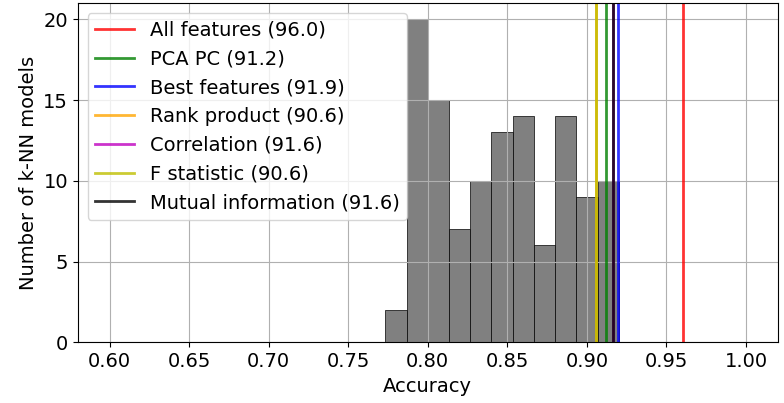
\includegraphics[width=\textwidth]{assets/results/feature-combinations/model-distr-fsel-k5-f3-TD-train.png}
        \caption{Time-domain features (train)}
    \end{subfigure}
    \hfill
    \begin{subfigure}[b]{0.48\textwidth}
        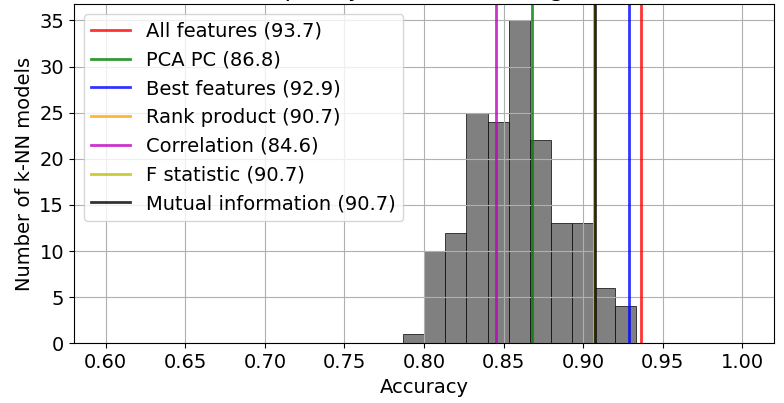
\includegraphics[width=\textwidth]{assets/results/feature-combinations/model-distr-fsel-k5-f3-FD-train.png}
        \caption{Frequency-domain features (train)}
    \end{subfigure}
    \hfill
    \begin{subfigure}[b]{0.48\textwidth}
        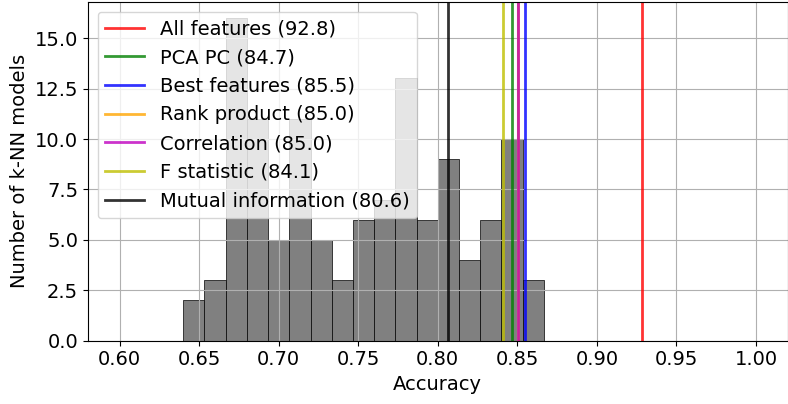
\includegraphics[width=\textwidth]{assets/results/feature-combinations/model-distr-fsel-k5-f3-TD-test.png}
        \caption{Time-domain features (test)}
    \end{subfigure}
    \hfill
    \begin{subfigure}[b]{0.48\textwidth}
        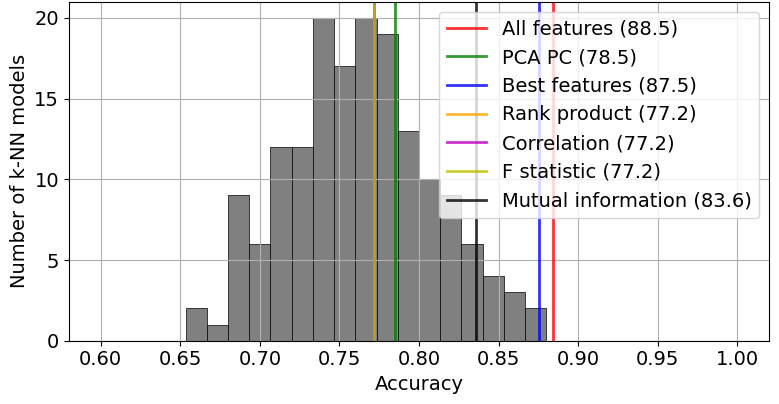
\includegraphics[width=\textwidth]{assets/results/feature-combinations/model-distr-fsel-k5-f3-FD-test.png}
        \caption{Frequency-domain features (test)}
    \end{subfigure}
    \caption{Model accuracy statistical distibutions with feature selection methods for three predictors (k = 5)}
    \label{fig:evaluation:fsel-model-distr}
\end{figure}

The entire accuracy distribution for the training and testing set for original labels is drawn in the form of the histogram (Fig.~\ref{fig:evaluation:fsel-model-distr}). The results of the chosen predictors are mapped out onto the distribution as vertical lines that stack up near the maximum for the time domain or disperse slightly above the median for the frequency domain. The accuracy of all features is unreachable for three feature subsets. Another noticeable difference between distributions is their shift down and greater spread in testing compared to training sets.

\begin{table}[]
\centering
\begin{adjustbox}{width=\textwidth}
\begin{tabular}{|l|r|r|}
\hline
\textbf{Method}    & \multicolumn{1}{l|}{\textbf{Median percentile {[}\%{]}}} & \multicolumn{1}{l|}{\textbf{Median accuracy {[}\%{]}}} \\ \hline
Rank product       & 88.97                                                    & 79.82                                                 \\ \hline
Mutual information & 91.81                                                    & 80.87                                                 \\ \hline
F statistic        & 86.90                                                    & 79.63                                                 \\ \hline
Correlation        & 84.49                                                    & 79.04                                                  \\ \hline
\end{tabular}
\end{adjustbox}
\caption{Feature selection methods evaluated in summary over all experimental conditions}
\label{tab:evaluation:compare-fsel-accuracy}
\end{table}

\begin{table}[]
\centering
\begin{adjustbox}{width=\textwidth}
\begin{tabular}{|l|r|r|r|}
\hline
                            & \multicolumn{1}{l|}{\textbf{Best in scenarios}} & \multicolumn{1}{l|}{\textbf{Scenarios {[}\%{]}}} & \multicolumn{1}{l|}{\textbf{Mean percentile {[}\%{]}}} \\ \hline
\textbf{Rank product}       & 94                                                     & 43.52                                            & 92.38 \\ \hline
\textbf{Mutual information} & 87                                                      & 40.28                                            & 91.79 \\ \hline
\textbf{Correlation}        & 26                                                      & 12.04                                             & 97.54 \\ \hline
\textbf{F statistic}        & 9                                                       & 4.16                                             & 96.10 \\ \hline
\textbf{$\Sigma$}           & 216                                                     & 100                                       & -                                                      \\ \hline
\end{tabular}
\end{adjustbox}
\caption{The experimental scenarios in which the method is found to be the best}
\label{tab:evaluation:best-selection-method}
\end{table}

\begin{figure}[t]
    \centering
    \begin{subfigure}[b]{0.48\textwidth}
        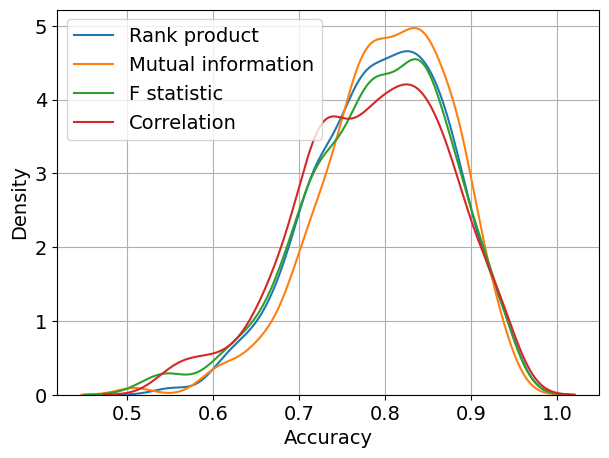
\includegraphics[width=\textwidth]{assets/results/feature-combinations/fsel-accuracy.png}
        \caption{Accuracy}
    \end{subfigure}
    \hfill
    \begin{subfigure}[b]{0.48\textwidth}
        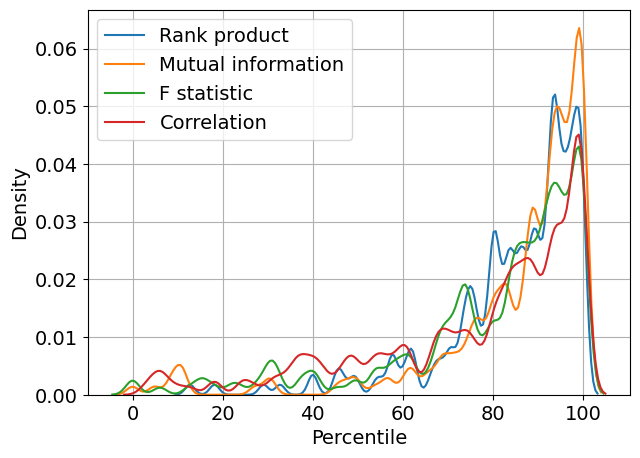
\includegraphics[width=\textwidth]{assets/results/feature-combinations/fsel-percentile.png}
        \caption{Percentile in distribution of accuracies}
    \end{subfigure}
    \caption{Quality of choice for feature selection methods}
    \label{fig:evaluation:kde-fsel-perecentile}
\end{figure}

\begin{figure}[t]
    \centering
    \begin{subfigure}[b]{0.24\textwidth}
        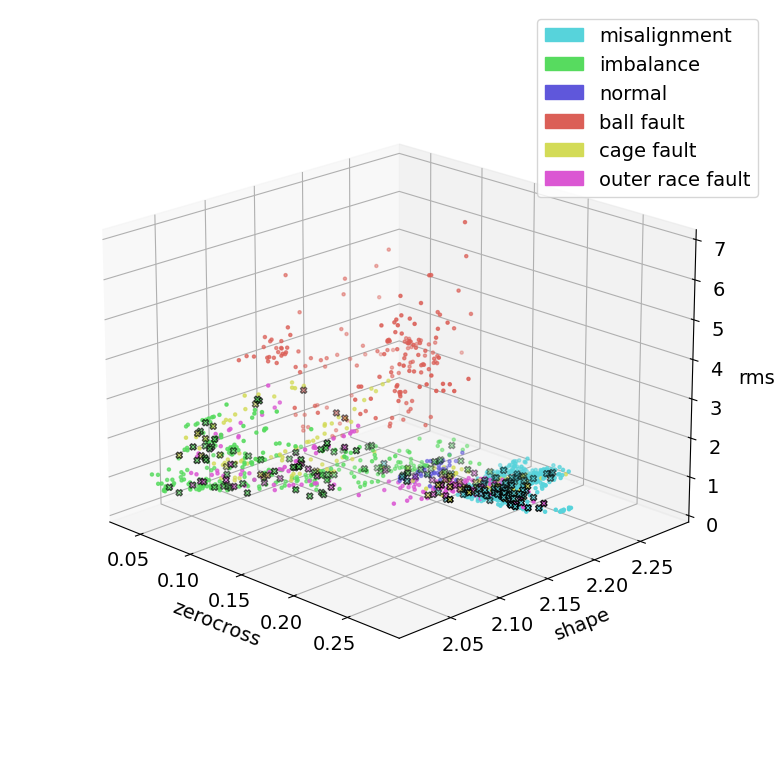
\includegraphics[width=\textwidth]{assets/results/labels/TD.png}
        \caption{TD [89.05\%]}
    \end{subfigure}
    \hfill
    \begin{subfigure}[b]{0.24\textwidth}
        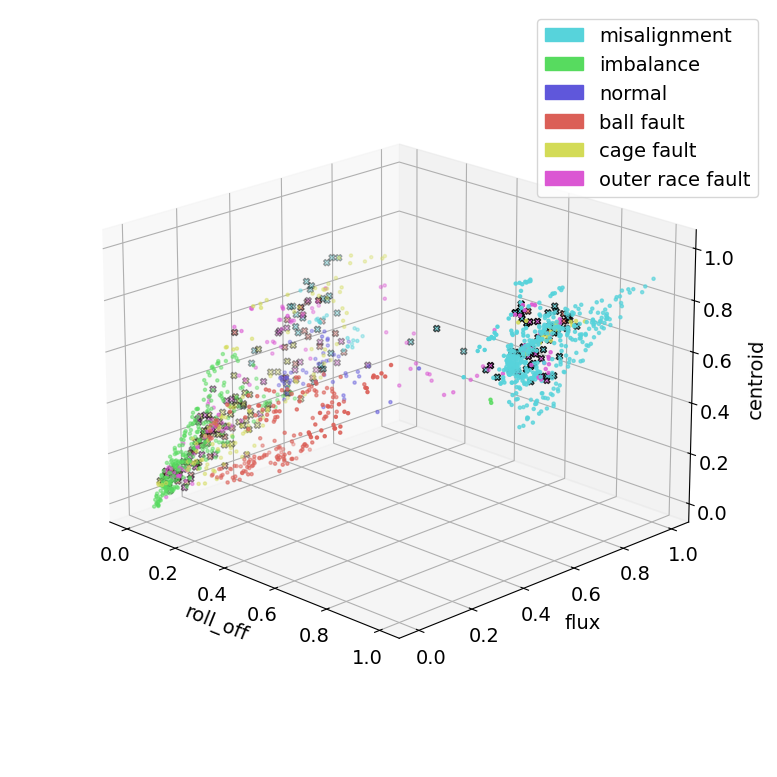
\includegraphics[width=\textwidth]{assets/results/labels/FD.png}
        \caption{FD [77.18\%]}
    \end{subfigure}
    \hfill
    \begin{subfigure}[b]{0.24\textwidth}
        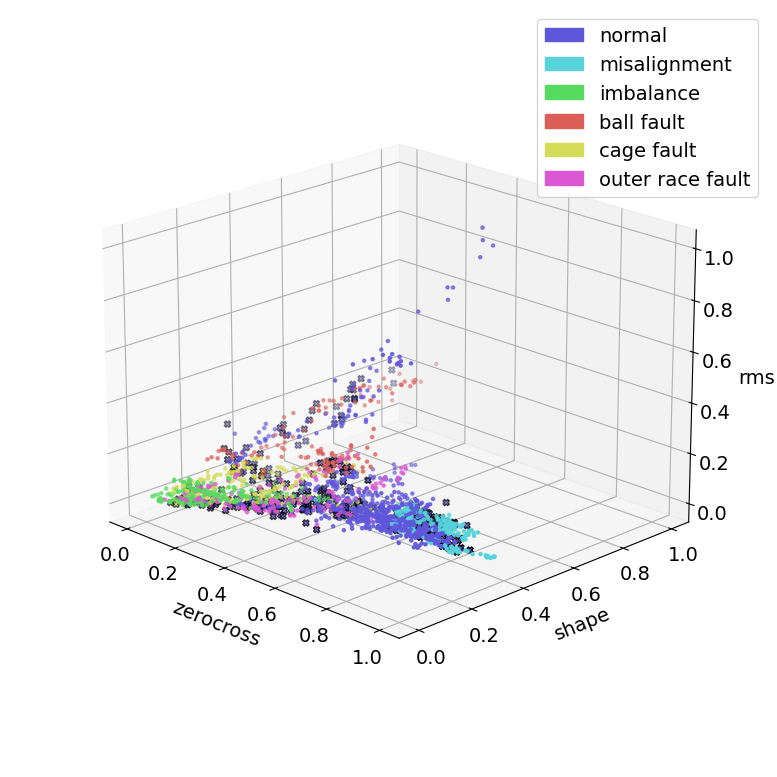
\includegraphics[width=\textwidth]{assets/results/labels/TD-severity.png}
        \caption{TD (s) [91.40\%]}
    \end{subfigure}
    \hfill
    \begin{subfigure}[b]{0.24\textwidth}
        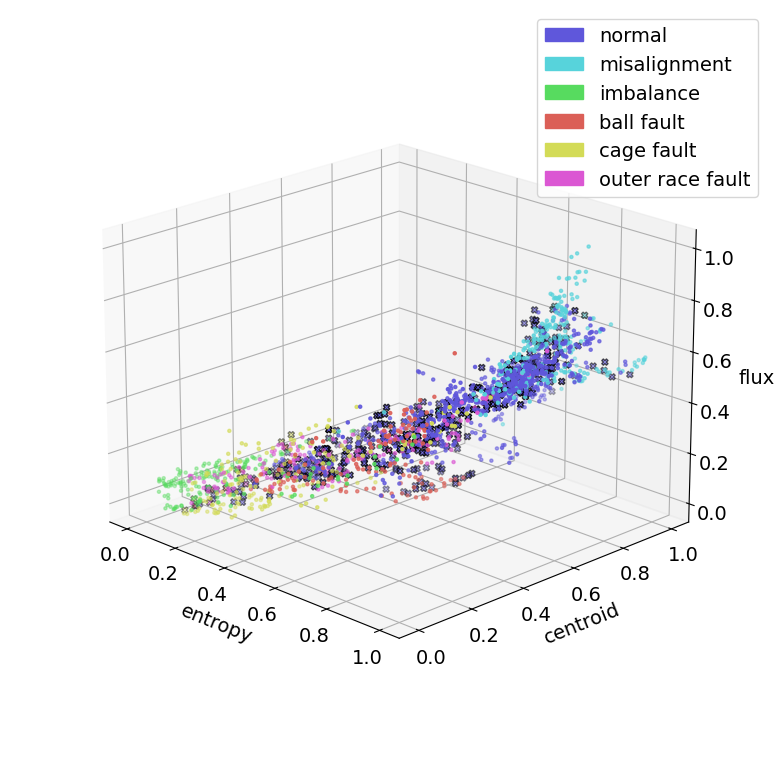
\includegraphics[width=\textwidth]{assets/results/labels/FD-severity.png}
        \caption{FD (s) [91.24\%]}
    \end{subfigure} 
    \caption{Three features in both domains chosen by rank product with prediction accuracy in brackets. Relabeled dataset is marked with (s)}
\end{figure}


Under 216 scenarios, the mutual information has better median accuracy (80.87\%) and distribution percentile (91.81\%) followed by rank product with an accuracy of 79.82\% of and percentile of 88.97\% (Tab.~\ref{tab:evaluation:compare-fsel-accuracy}). The scenarios are composed of 24 base dataset modifications and options for hyperparameters k-value and number of features. 

The rank product was the best method in the majority of 43.52\% scenarios. Mutual information comes second in 40.28\% cases, where it is deemed the best strategy (Tab.~\ref{tab:evaluation:best-selection-method}). The median accuracy in selected cases is also better for rank product 92.38\% compared to 91.79\% mutual information. 

Kernel density estimate plot (Fig.~\ref{fig:evaluation:kde-fsel-perecentile}) shows the distribution of accuracies for the selection methods and percentiles for predictor subsets they chose. The feature selection usually picks variables so that they stay in the upper quartile of the distribution above the 75\% percentile. The median accuracy of all methods is around the vicinity of 80\%.

The features chosen by rank product are visualized as a three-dimensional scatter plot. The colors of data points represent correct labels with ex marks for misses. The scales on graph axes are inverse transformed of the min-max scaler. The visualization of predicted groups suggests another transform should be applied to even out the distances and handle the outliers.


\subsection{Incremental learning}
Online learning imitates hardened conditions for machinery diagnostics that appear in deployment. Delayed provision or omission of actual labels undoubtedly degrades the reliability of the classification. The question is how quickly the accuracy approaches the optimal one from the nearest neighbors trained in batch and what is the effect on the classifier from routine difficulties associated with the continous labeling process.

\begin{figure}[ht]
    \centering
    \begin{subfigure}[b]{0.32\textwidth}
        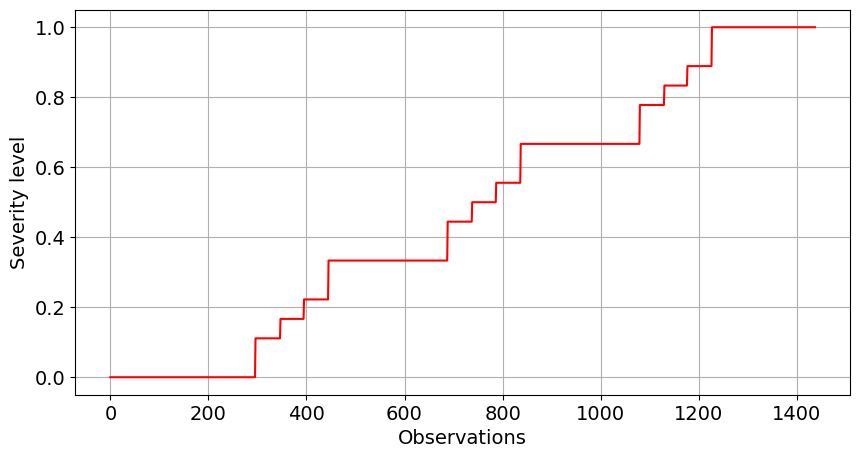
\includegraphics[width=\textwidth]{assets/results/incremental-learning/severity-levels.png}
        \caption{Relative severity levels}
        \label{fig:design:online-count-severity-level}
    \end{subfigure}
    \hfill
    \begin{subfigure}[b]{0.32\textwidth}
        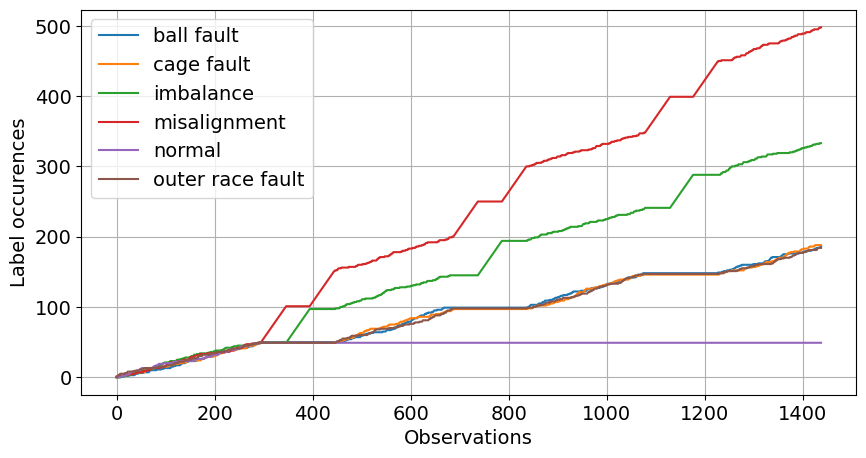
\includegraphics[width=\textwidth]{assets/results/incremental-learning/order-natural.png}
        \caption{Original labels}
        \label{fig:design:online-event-order}
    \end{subfigure}
    \hfill
    \begin{subfigure}[b]{0.32\textwidth}
        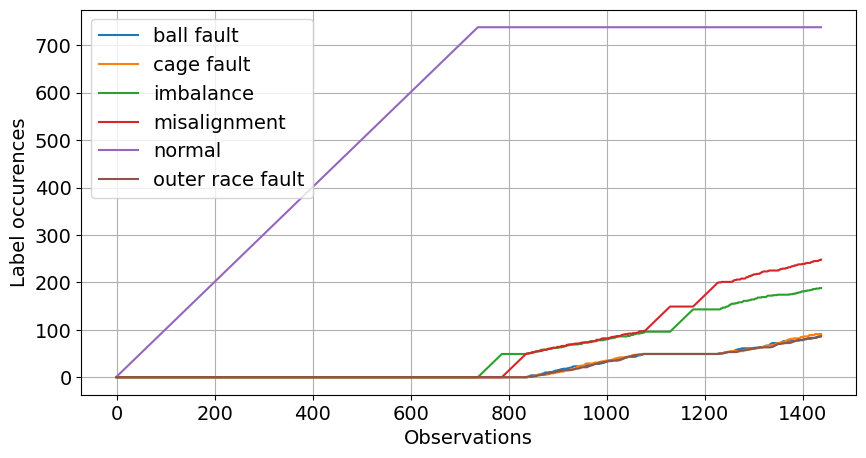
\includegraphics[width=\textwidth]{assets/results/incremental-learning/order-severity.png}
        \caption{High severity labels}
         \label{fig:design:online-event-order-severity}
    \end{subfigure}
    \caption{Ordering of faults in dataset according to relative severity levels}
\end{figure}

The k-NN models in incremental learning experiments learn on the same base training dataset as in batch learning for bearing A with complete sets of extracted features. In this manner, we can compare the training accuracies in the last sample for both models. Online learning metrics are evaluated by progressive valuation on a dataset that is left unbalanced.

The \textbf{stream of events} is ordered by rising severity levels (Fig.~\ref{fig:design:online-count-severity-level}), which ensures steady increments in label counts throughout the simulation (Fig.~\ref{fig:design:online-event-order}). The same sorting approach is applied to the dataset where low-severity faults are annotated as baseline. During most of its lifespan, the machine simulator looks to be in a fine operating state. Near the end of the simulation, faults start to develop (Fig.~\ref{fig:design:online-event-order-severity}). These artificially streamed event sequences are a bit unrealistic because all types of faults never begin to appear simultaneously with equal strengths. It is meant to approximate the gradual overall degradation of the machine.

A significant change in the data stream occurs after 294 out of 1438 observations (or after 737 for high severity faults) when all 49 (or 737) normal conditions are consumed in the training process. Counters of other faults show that predictions are skewed towards more represented imbalance and misalignement. The uneven evolution of categories in a stream impacts the development of accuracy in the remaining experiments. The test accuracies of comparable batch models from the three best features are 85.47\% (TD), 87.52\% (FD), 91.71\% (TD severity), and 91.94\% (FD severity).

\begin{figure}[]
    \centering
    \begin{subfigure}[b]{0.48\textwidth}
        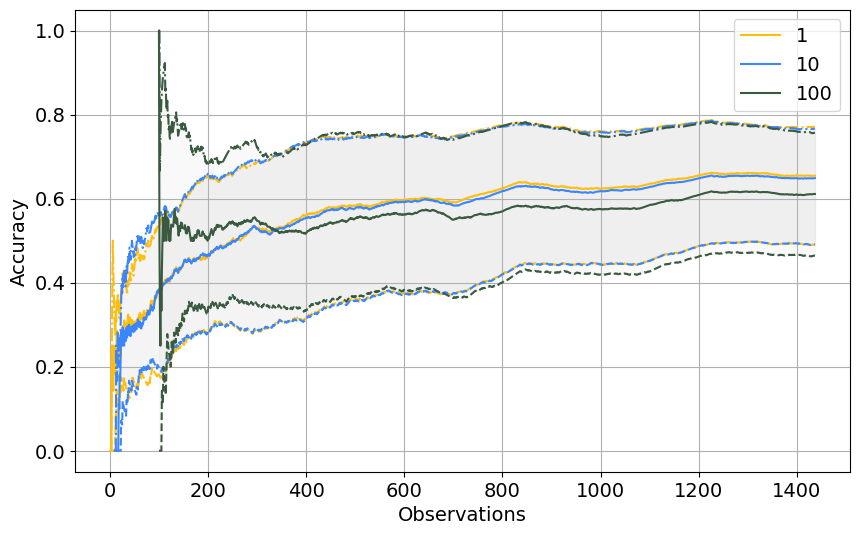
\includegraphics[width=\textwidth]{assets/results/incremental-learning/tumbling-TD.png}
        \caption{Time-domain features}
    \end{subfigure}
    \hfill
    \begin{subfigure}[b]{0.48\textwidth}
        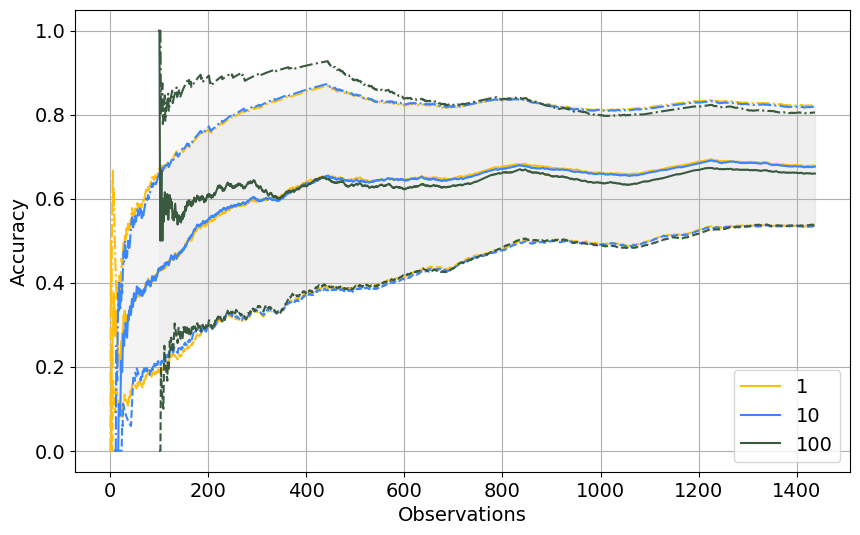
\includegraphics[width=\textwidth]{assets/results/incremental-learning/tumbling-FD.png}
        \caption{Frequency-domain features}
    \end{subfigure}
    \hfill
    \begin{subfigure}[b]{0.48\textwidth}
        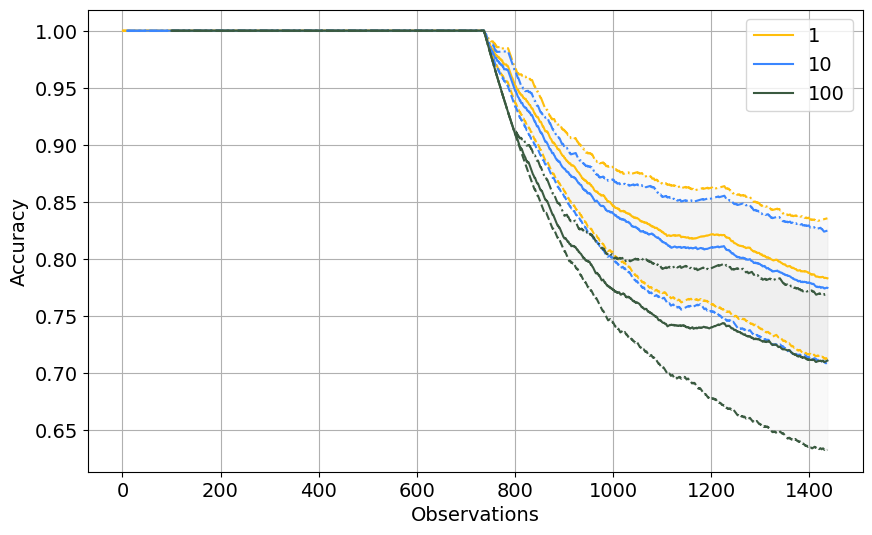
\includegraphics[width=\textwidth]{assets/results/incremental-learning/tumbling-TD-severity.png}
        \caption{Time-domain features (severity)}
    \end{subfigure}
    \hfill
    \begin{subfigure}[b]{0.48\textwidth}
        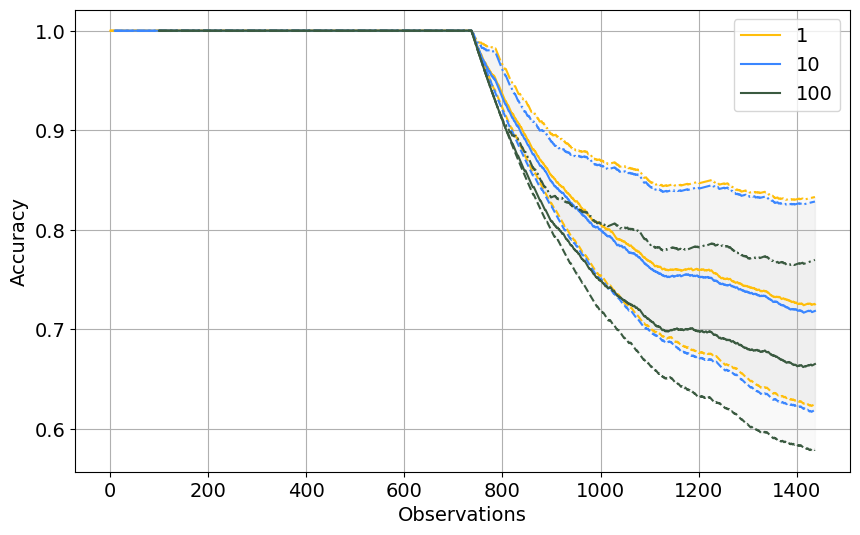
\includegraphics[width=\textwidth]{assets/results/incremental-learning/tumbling-FD-severity.png}
        \caption{Frequency-domain features (severity)}
    \end{subfigure} 
    \caption{Tumbling window during incremental learning of lengths 1, 10, 100}
    \label{fig:evaluation:tumbling-window-online}
\end{figure}

\begin{figure}[]
    \centering
    \begin{subfigure}[b]{0.48\textwidth}
        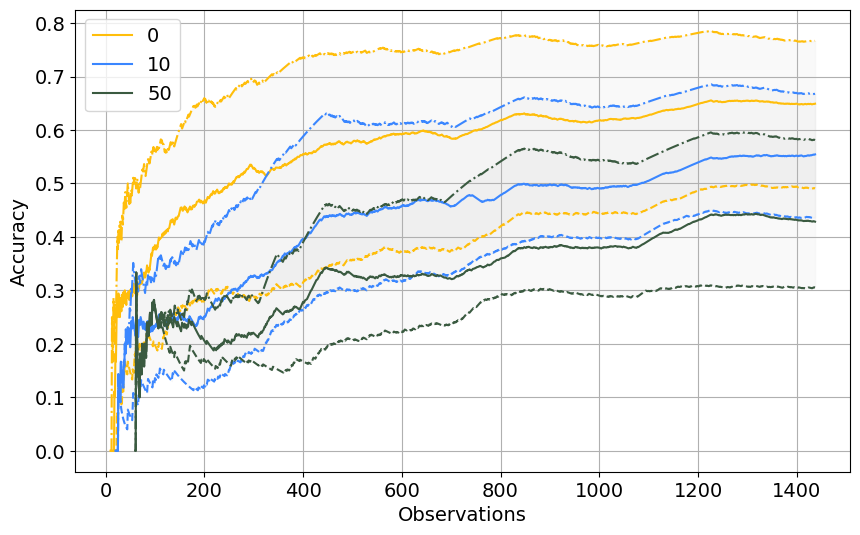
\includegraphics[width=\textwidth]{assets/results/incremental-learning/skip-label-TD.png}
        \caption{Time-domain features}
    \end{subfigure}
    \hfill
    \begin{subfigure}[b]{0.48\textwidth}
        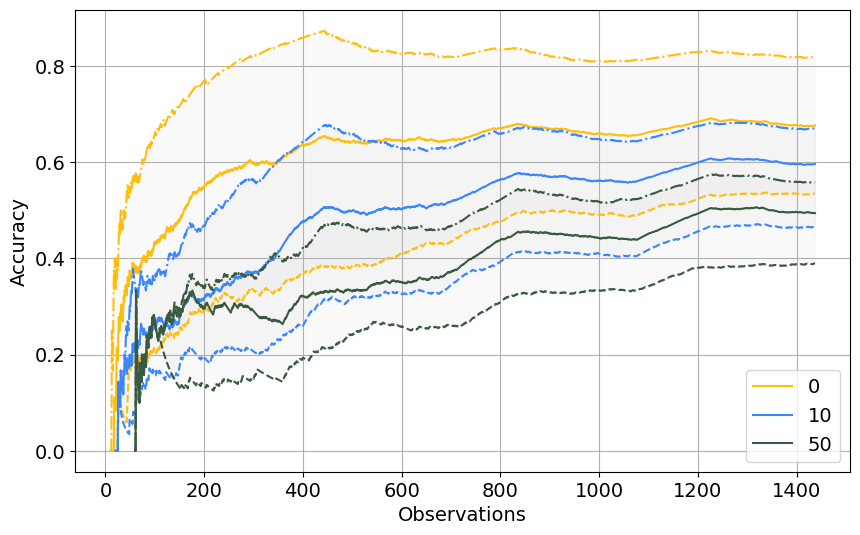
\includegraphics[width=\textwidth]{assets/results/incremental-learning/skip-label-FD.png}
        \caption{Frequency-domain features}
    \end{subfigure}
    \hfill
    \begin{subfigure}[b]{0.48\textwidth}
        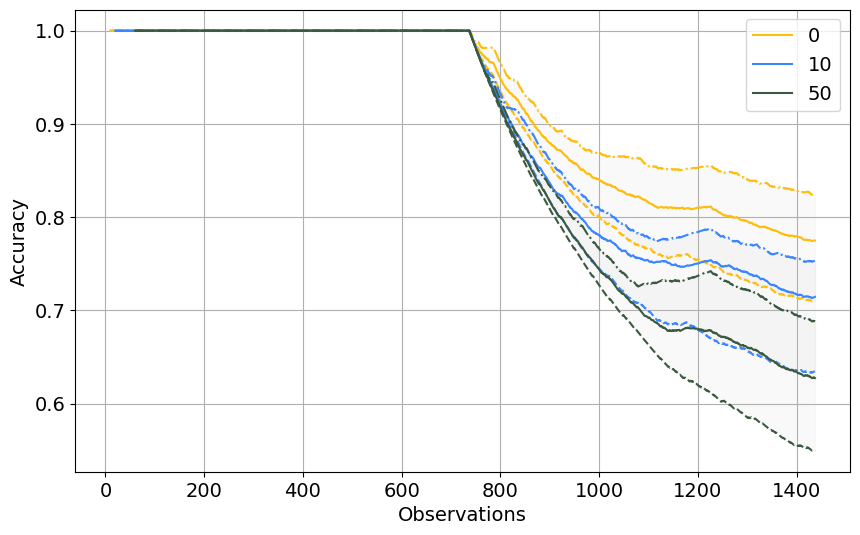
\includegraphics[width=\textwidth]{assets/results/incremental-learning/skip-label-TD-severity.png}
        \caption{Time-domain features (severity)}
    \end{subfigure}
    \hfill
    \begin{subfigure}[b]{0.48\textwidth}
        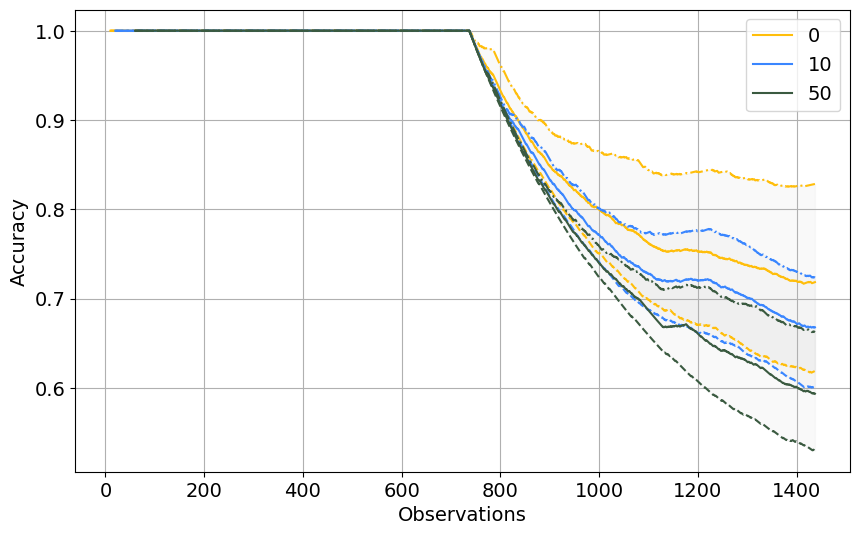
\includegraphics[width=\textwidth]{assets/results/incremental-learning/skip-label-FD-severity.png}
        \caption{Frequency-domain features (severity)}
    \end{subfigure} 
    \caption{Omission of labels during incremental learning with tumbing window of length 10 and gaps of size 0, 10, and 50 samples}
    \label{fig:evaluation:label-skips-online}
\end{figure}

During gradual learning, the correct labels are supplied in bulk at a fixed period. Labeling delay in \textbf{tumbling window} decreases towards the window's end. Figure~\ref{fig:evaluation:tumbling-window-online} plots the evolution of the k-NN model's distribution of accuracy for windows of size 1, 10, and 100 observations. The models consist of three predictors and use five neighbours for prediction. Each window length is described with three curves of identical colour. The median is drawn with a solid line, the maximum with a dash-dotted line, and the minimum with a dashed line.

Initial zero accuracy is caused by a warming-up period in data collection during the span of the first few windows. The true labels are unknown at that point. After just a handful of windows in the beginning, accuracy jumps above 60\% for the best triplet of attributes and stabilizes after 400 observations. In an alternative labeling scheme, the accuracy for one class is 100\% and only after encountering other fault types, it decreases to a level above 75\% for the best set.

The top accuracies after sequentially seeing samples in the longest tumbling windows of 100 observations are 75.71\% (TD), 76.98\% (FD), 76.98\% (TD severity), and 80.56\% (FD severity). The degradations in accuracy when compared to the batch model are by 9.76\% (TD), 10.54\% (FD), 14.73\% (TD severity), and 11.38\% (FD severity). The effect of severe performance hit could be attributed to unbalanced data based on the analysis chapter. The online multiclass oversampling method would need to be inserted into the pipeline to prove this hypothesis.

Labeling every \nth{10} sample (10\% of the dataset) with a tumbling window of 10 samples reduces maximum accuracy for the three-predictor model compared to data points without gaps in labels. Time-domain features it is decreased by 9.9\% to 66.78\%, and by 14.93\% for frequency-domain features to 67.00\% (Fig.~\ref{fig:evaluation:label-skips-online}). More annotations can be scrapped in the case of a relabeled dataset where keeping just 0.02\% of the class labels produces a decrease by 13.7\% to 68.79\% for time domain attributes, and by 16.59\% to 66.25\% for frequency domain attributes.


\section{Industrial dataset analysis}
The latter part of the solution evaluation focuses on signal properties of vibrations from air compressors, water pumps, and electric induction motors. At first, the accelerometer data logger functionality is tested, and its precision is checked up in the known situations. Our custom dataset is compiled from collected measurements during regular operations of machines. The behaviour of different machines is compared using static frequency estimation and a time-frequency spectrogram. The methodology is carried out to diagnose the current status of water pumps. The presence of fault is confronted with sensor logs from the pump vendor.

\subsection{Data logger verification}
Data logger capabilities were verified by capturing vibrations on the back of the plastic casing for the electric motor of the standing fan. The recording is able to run continuously for more than one minute without dropping any samples. The amplitude range after conversion is constrained in the expected range (Fig.~\ref{fig:evaluation:logger-waveform}). The same amplitudes were obtained previously on a proof-of-concept device using analog accelerometer ADXL335 on Beaglebone Black, albeit with lower sensitivity.

\begin{figure}[h]
    \centering
    \begin{subfigure}[b]{0.49\textwidth}
        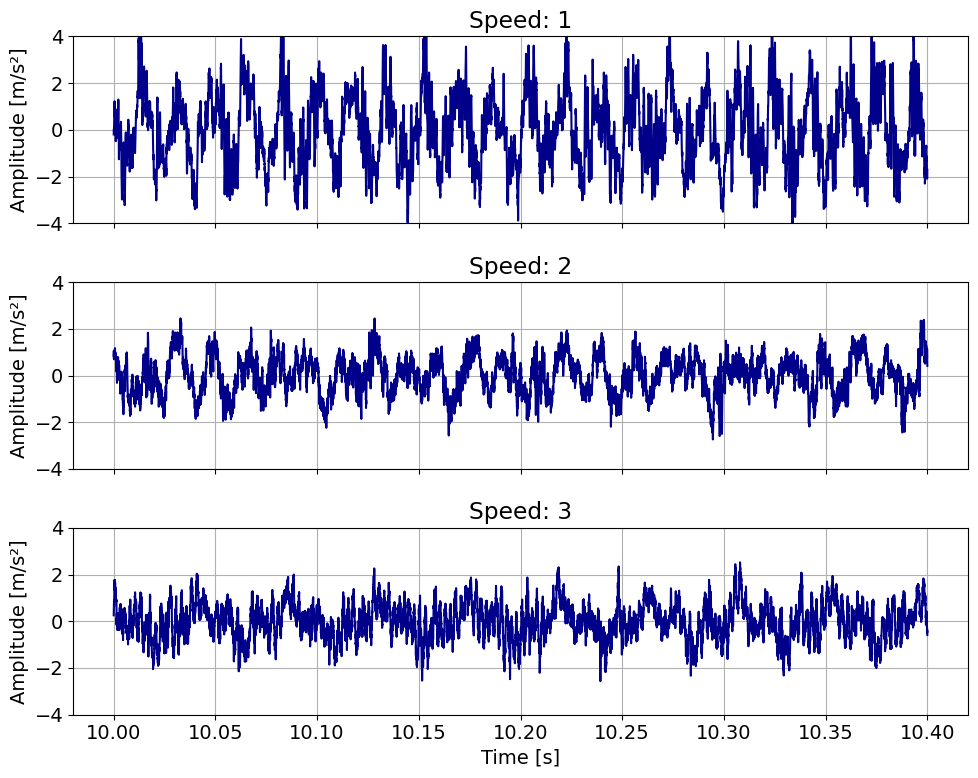
\includegraphics[width=\textwidth]{assets/results/standing-fan/waveform.png}
        \caption{Time waveform}
        \label{fig:evaluation:logger-waveform}
    \end{subfigure}
    \hfill
    \begin{subfigure}[b]{0.49\textwidth}
        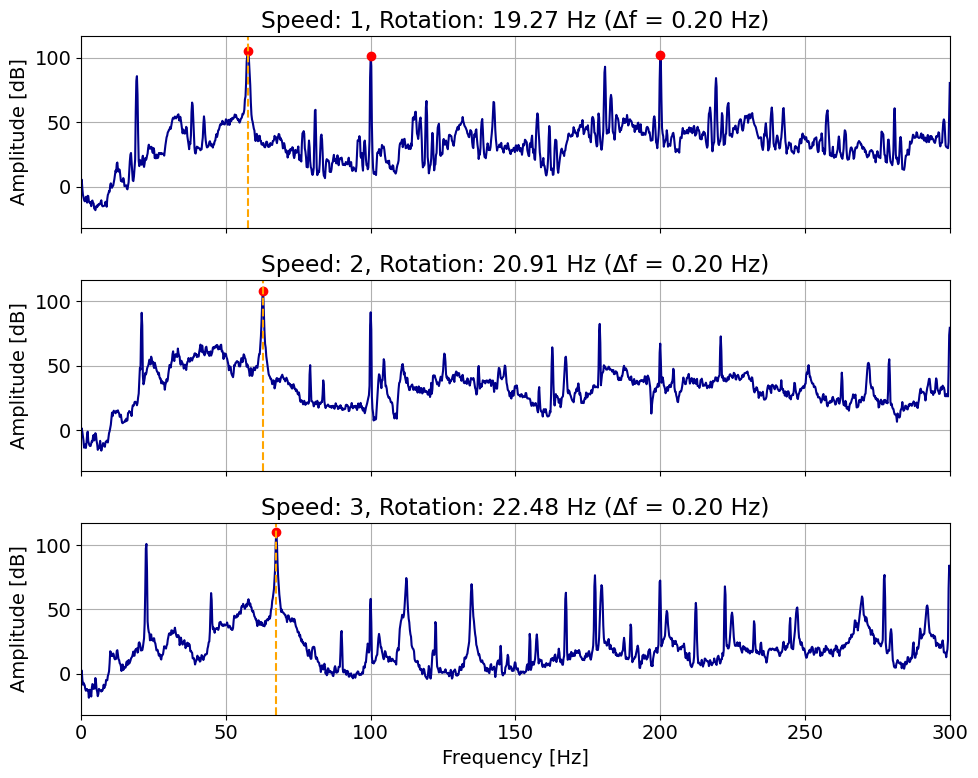
\includegraphics[width=\textwidth]{assets/results/standing-fan/standing-fan-accel.png}
        \caption{Estimation of rotation speed}
        \label{fig:evaluation:logger-fan-speed}
    \end{subfigure}
    \caption{Vibrations from the back of a standing fan in the radial direction}
\end{figure}

Time waveform captures mostly regular patterns of oscillatory motion  (Fig.~\ref{fig:evaluation:logger-waveform}). At slower speeds, the vibrations are higher because the fan is less stable and wobbles around the support. Timestamps from the sensor calibrate the sampling frequency from the theoretical 26667 Hz to the actual 26866 Hz. The estimate of fan rotational speed (Fig.~\ref{fig:evaluation:logger-fan-speed}) is accurate within the margin of error.

\subsection{Signal waveforms}
\begin{figure}[h]
    \centering
    \begin{subfigure}[b]{0.32\textwidth}
        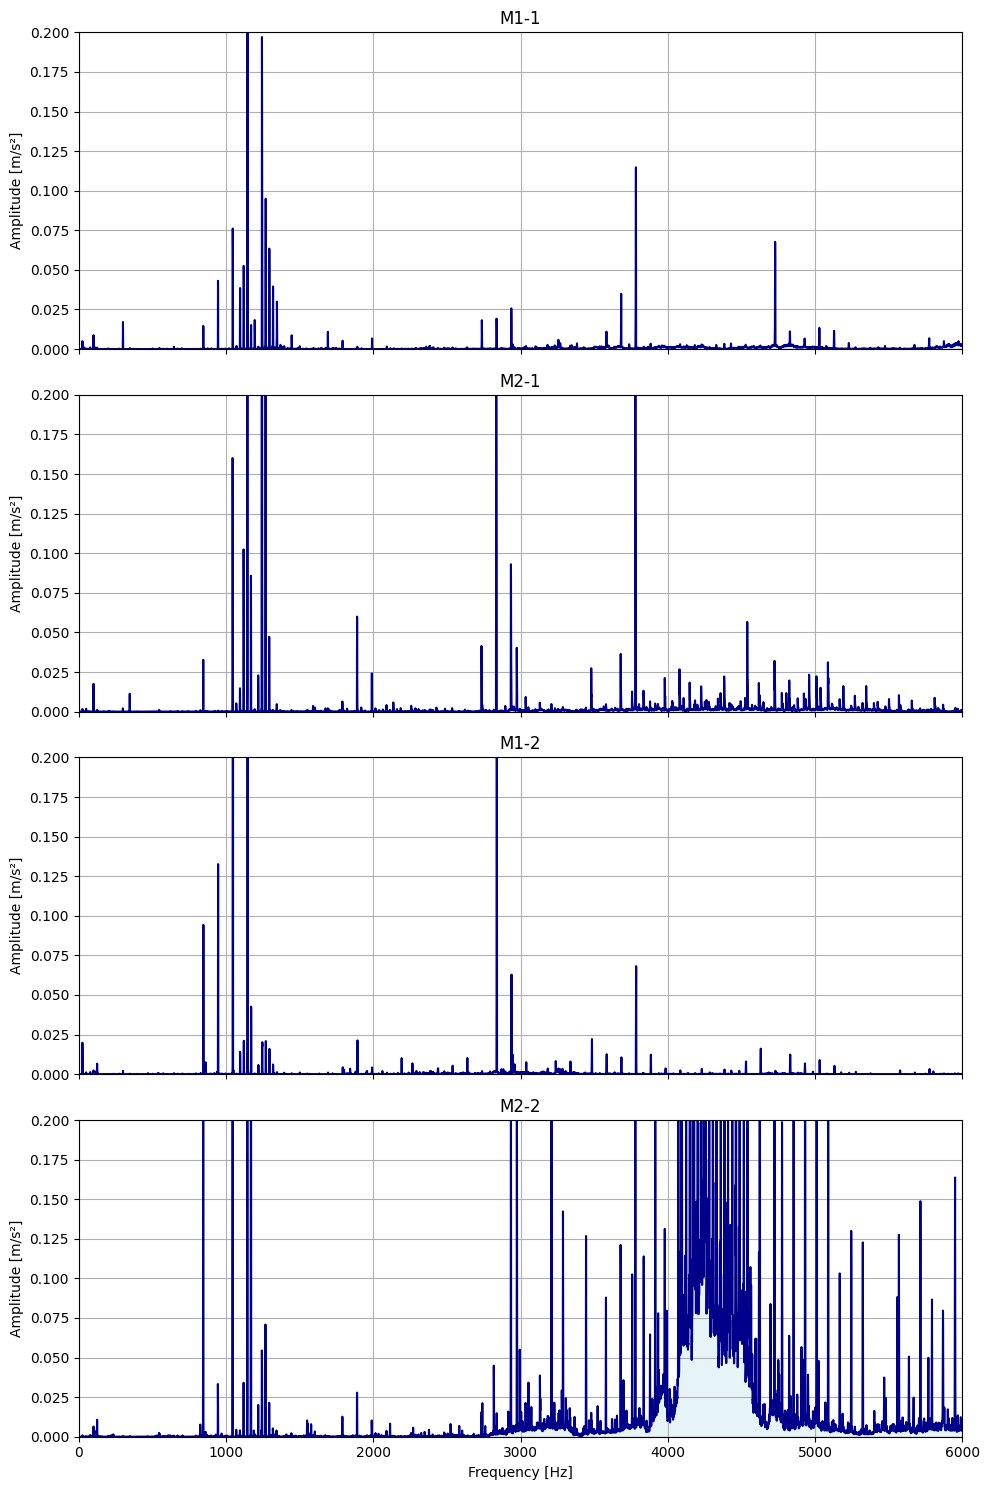
\includegraphics[width=\textwidth]{assets/results/eda/frequency-spectrum-motors.png}
        \caption{Motors}
    \end{subfigure}
    \hfill
    \begin{subfigure}[b]{0.32\textwidth}
        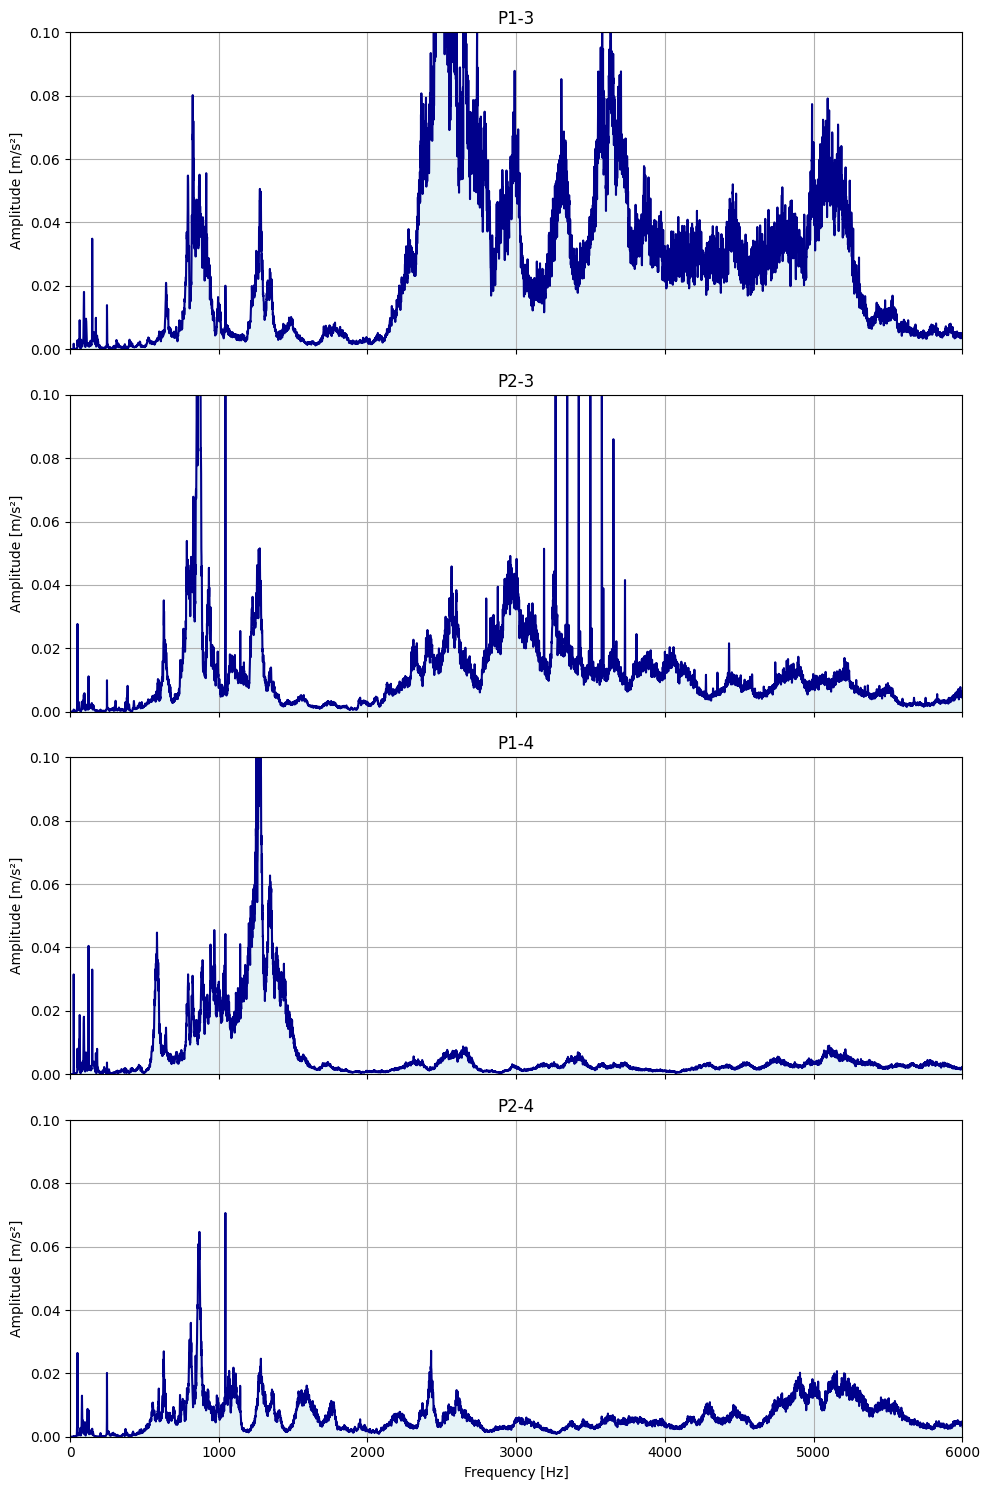
\includegraphics[width=\textwidth]{assets/results/eda/frequency-spectrum-pumps.png}
        \caption{Pumps}
    \end{subfigure}
    \hfill
    \begin{subfigure}[b]{0.32\textwidth}
        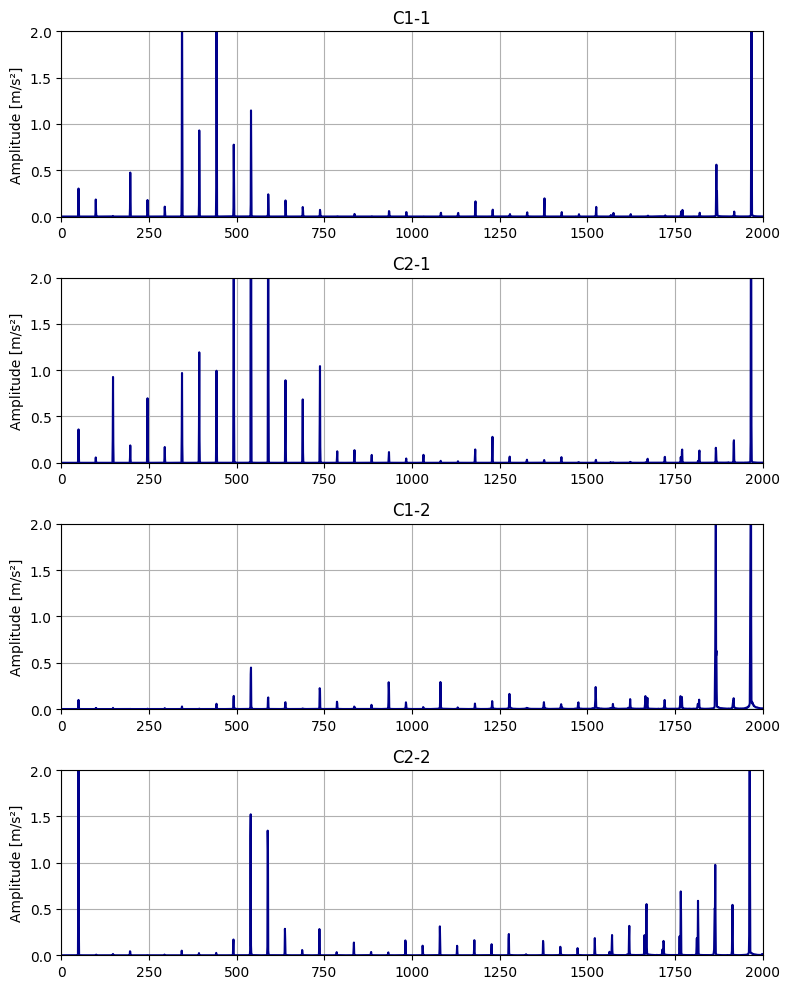
\includegraphics[width=\textwidth]{assets/results/eda/frequency-spectrum-compressors.png}
        \caption{Compressors}
    \end{subfigure} 
    \caption{Wideband frequency waveform of machinery vibartions in Pump dataset}
    \label{fig:evaluation:wideband-frequencies}
\end{figure}

The overview of wideband vibration frequency spectra from various sensor placements shows clear distinctions among the machines. The recordings in Figure~\ref{fig:evaluation:wideband-frequencies} present consistent shapes of waveforms found during repeated trials. The spectra are Welch's average of 32768 long windows with 50\% overlap over minute of recording.

The electric motor signals are polluted by noise from the wind blowing out of a large cooling fan at the back of the motor. The M2 in place two compared to M1 has elevated amplitudes above 4 kHz. The pumps have richer signal content, likely due to the flow of water split into several frequency bands. The outer bearing (4) has a more attenuated amplitude above 1.5 kHz than the inner bearing (3). The P2 exhibits less vibration in comparable bands in general. The compressor casing produces a series of harmonics of rotational frequency, which are stronger near the scroll and suction valve than near the base.

\begin{table}[h]
\centering
\begin{tabular}{|l|r|r|r|}
\hline
\textbf{Placement}     & \multicolumn{1}{l|}{\textbf{M1}} & \multicolumn{1}{l|}{\textbf{M2}} & \multicolumn{1}{l|}{\textbf{P3, P4}} \\ \hline
\textbf{Bearing}       & \multicolumn{1}{l|}{6319-C3}            & \multicolumn{1}{l|}{6324-C3}            & \multicolumn{1}{l|}{6317-2Z}                  \\ \hline
\textbf{Rolling elements $n$}           & 8                                       & 8                                       & 8                                             \\ \hline
\textbf{Rotational speed $f_s$ {[}rpm{]}}         & 1493                                    & 1493                                    & 1493                                          \\ \hline
\textbf{Inner diameter $d$ {[}mm{]}}  & 33.12                                   & 41.28                                   & 30.00                                         \\ \hline
\textbf{Outer diameter$D$ {[}mm{]}}  & 147.5                                   & 190.0                                   & 132.5                                         \\ \hline
\textbf{Contact angle $\beta$}       & 0                                       & 0                                       & 0                                             \\ \hline
\textbf{RPM {[}Hz{]}}  & 24.88                                   & 24.88                                   & 24.88                                         \\ \hline
\textbf{BPFO {[}Hz{]}} & 77.18                                   & 77.91                                   & 77.00                                         \\ \hline
\textbf{BPFI {[}Hz{]}} & 121.88                                  & 121.16                                  & 122.07                                        \\ \hline
\textbf{BSF {[}Hz{]}}  & 58.20                                   & 59.97                                   & 57.77                                         \\ \hline
\textbf{FTF {[}Hz{]}}  & 9.65                                    & 9.74                                    & 9.63                                          \\ \hline
\end{tabular}
\caption{Bearing characteristic harmonic frequencies of pumps and their motors}
\label{tab:evaluation:bearing-freq-pump}
\end{table}

\begin{figure}[h]
    \centering
    \begin{subfigure}[b]{0.24\textwidth}
        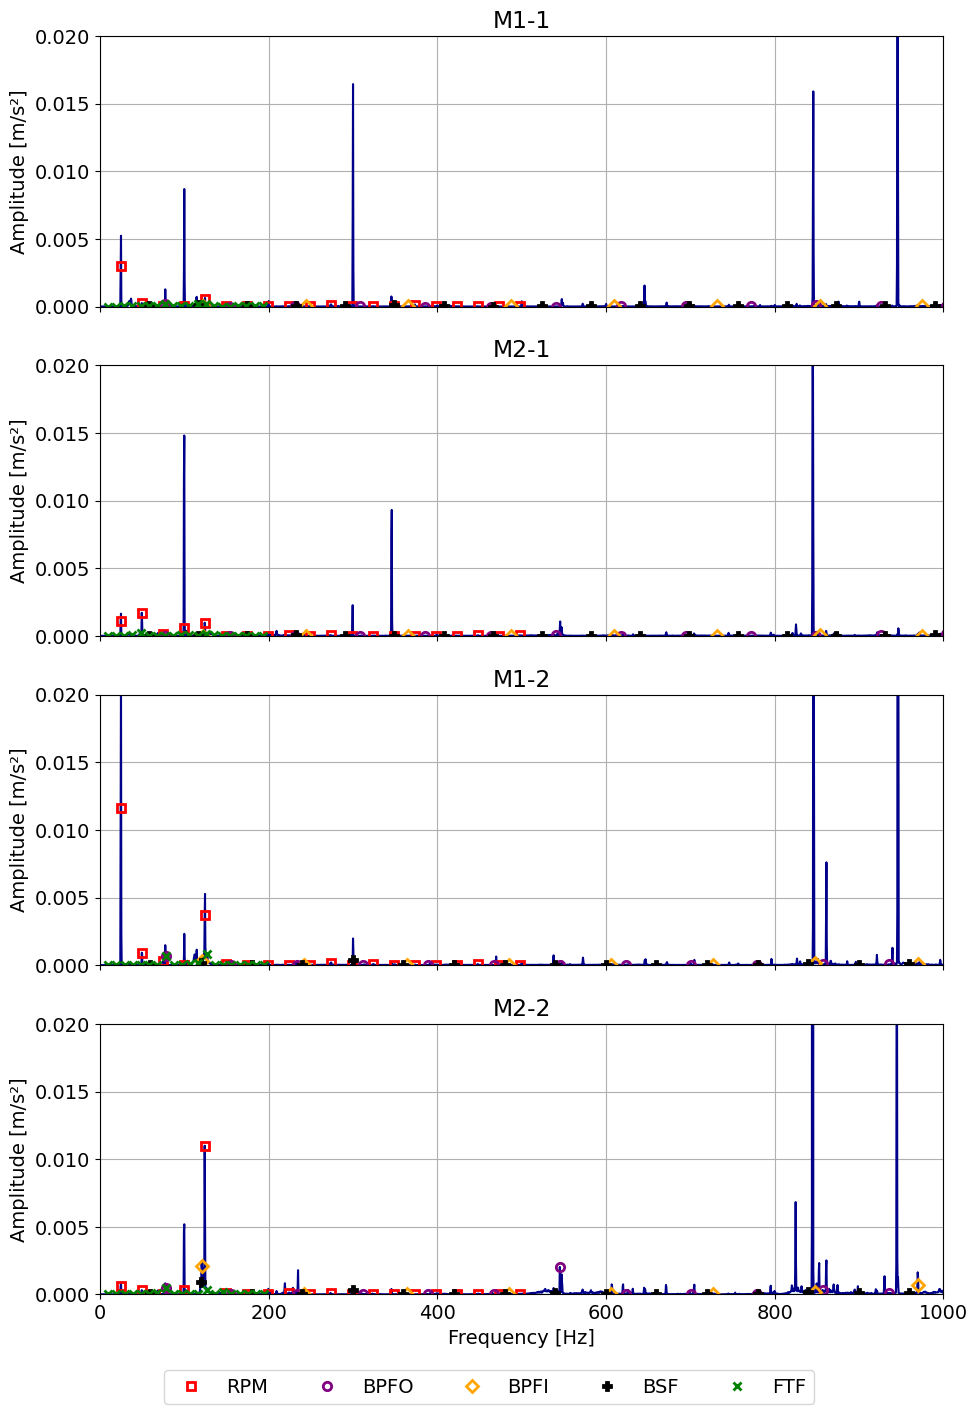
\includegraphics[width=\textwidth]{assets/results/defects/motors.png}
        \caption{Motors}
    \end{subfigure}
    \hfill
    \begin{subfigure}[b]{0.24\textwidth}
        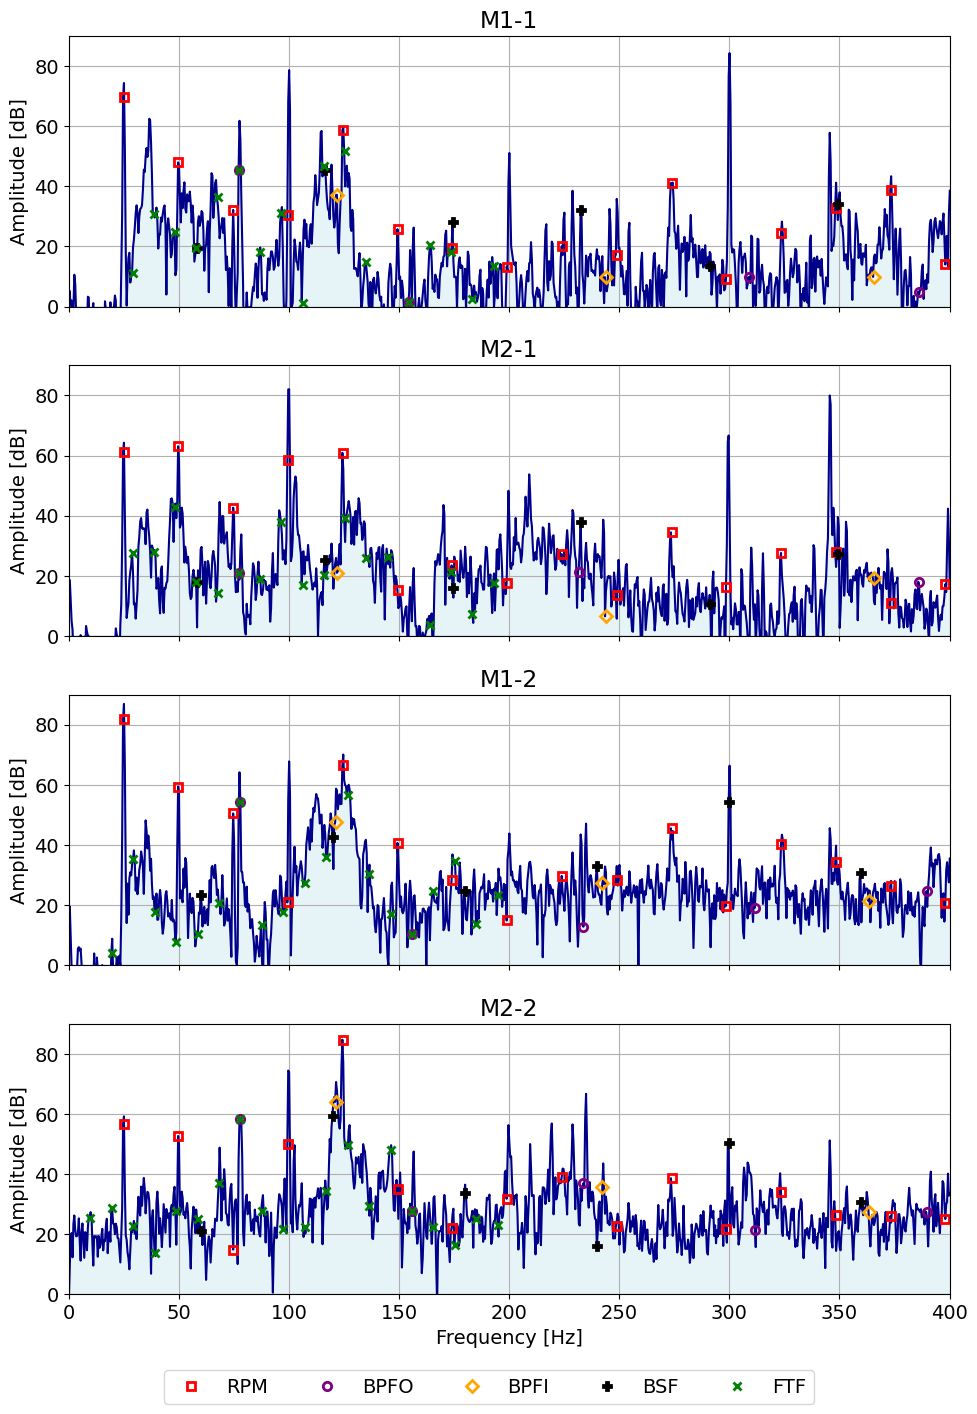
\includegraphics[width=\textwidth]{assets/results/defects/motors-dB.png}
        \caption{Pumps}
    \end{subfigure}
    \begin{subfigure}[b]{0.24\textwidth}
        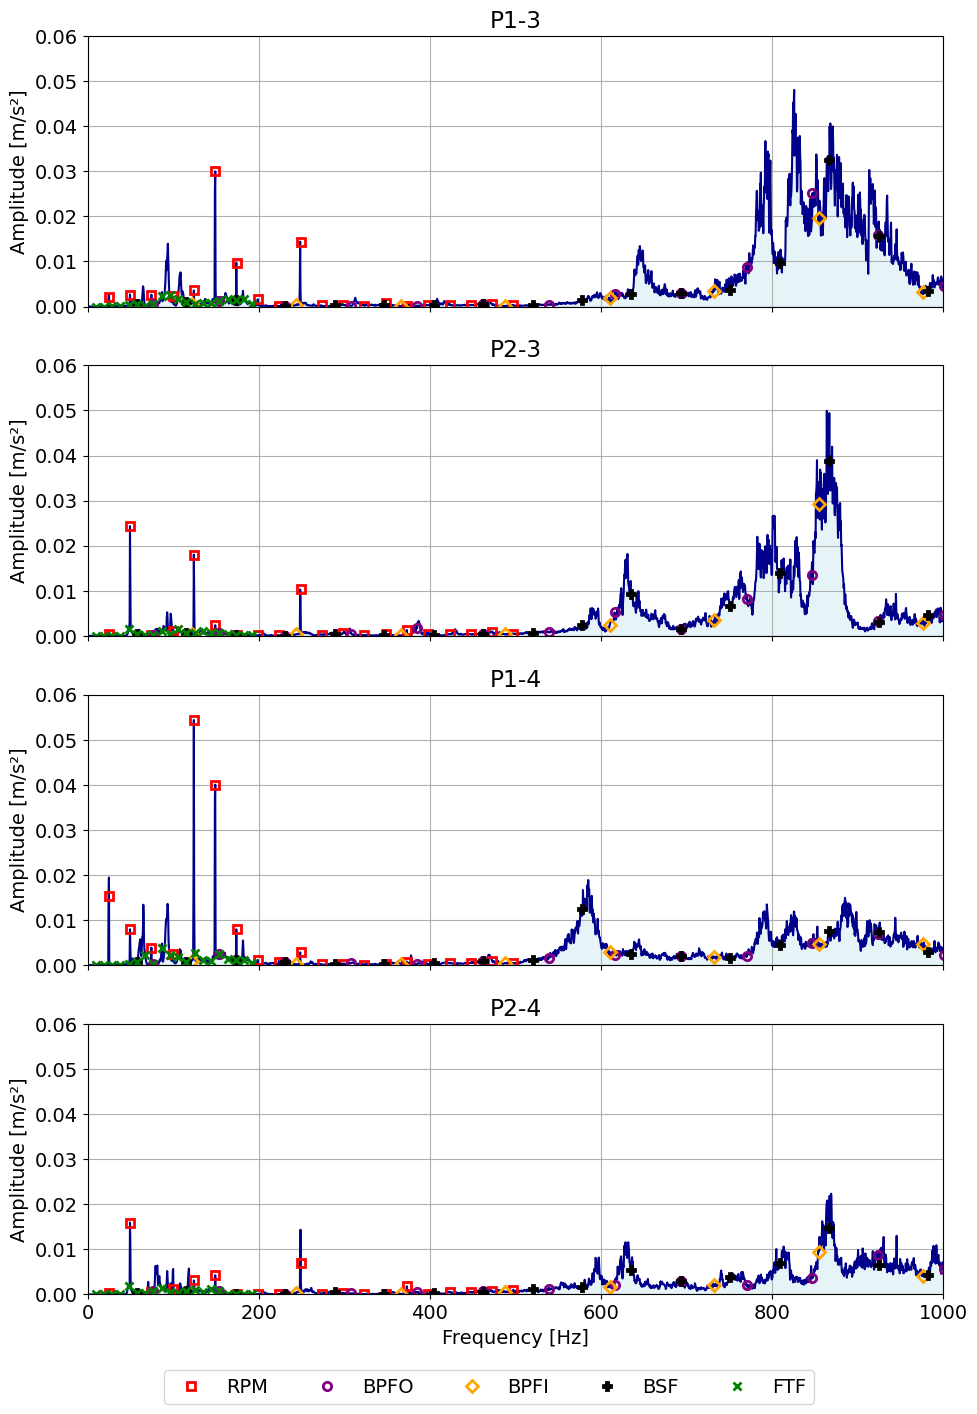
\includegraphics[width=\textwidth]{assets/results/defects/pumps.png}
        \caption{Motors}
    \end{subfigure}
    \hfill
    \begin{subfigure}[b]{0.24\textwidth}
        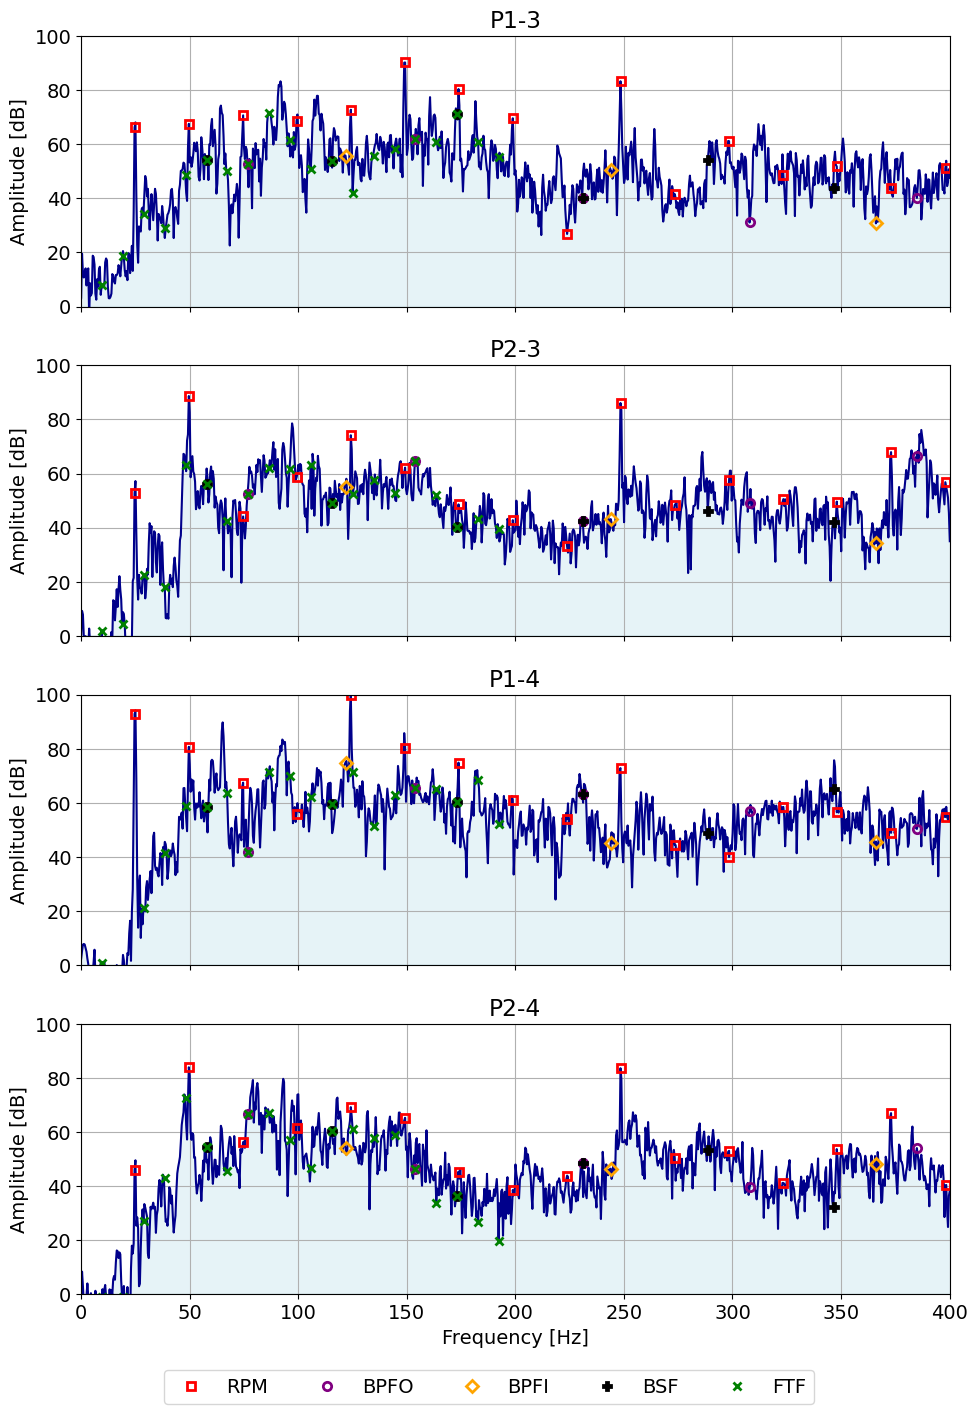
\includegraphics[width=\textwidth]{assets/results/defects/pumps-dB.png}
        \caption{Pumps dB}
    \end{subfigure}
    \caption{Characteric bearing frequencies of pumps}
    \label{fig:evaluation:bearing-freq}
\end{figure}

Domain experts recommended the procedure for fault identification by calculation of bearing characteristic frequencies (Tab.~\ref{tab:evaluation:bearing-freq-pump}), and then they approved the following results. Figure~\ref{fig:evaluation:bearing-freq} identifies harmonics of rotational speed and BPFO frequency in every machine and BPFI for M2-2. It can be assumed that those frequencies will be the reason for their damage in the future. The absolute acceleration is minuscule in current frequency bands and year-long sensor log of rms velocity (Fig~\ref{fig:evaluation:ksb-guard-rms-vibartions}).

\begin{figure}[h]
    \centering
    \begin{subfigure}[b]{0.49\textwidth}
        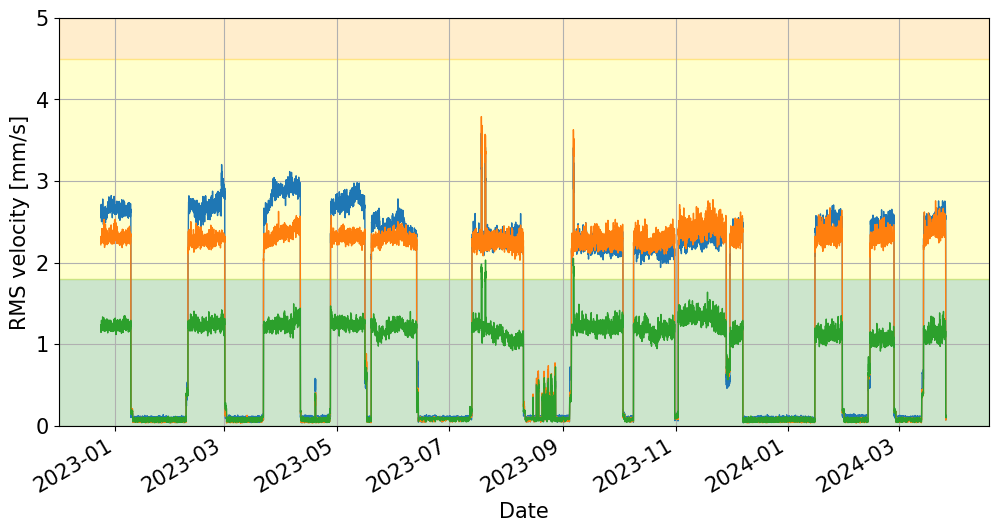
\includegraphics[width=\textwidth]{assets/results/ksb-cloud/p1.png}
        \caption{Pump P1}
    \end{subfigure}
    \hfill
    \begin{subfigure}[b]{0.49\textwidth}
        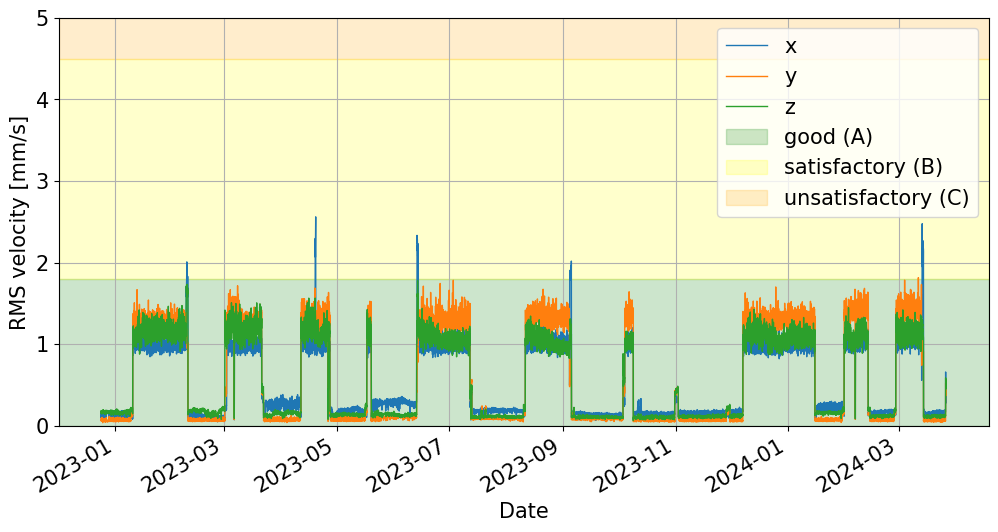
\includegraphics[width=\textwidth]{assets/results/ksb-cloud/p2.png}
        \caption{Pump P2}
    \end{subfigure}
    \caption{Vibration rms levels for a period over a year from KSB Guard}
    \label{fig:evaluation:ksb-guard-rms-vibartions}
\end{figure} 

Therefore, the current results suggest that the bearings are in flawless condition. During the over five years the pump has been in service, there is not one instance of bearing fault due to rated lifespan and yearly prophylactic maintenance. This underscores the difficulty of the scarcity of non-faulty states in industrial environments. The monitoring is better suited for situations without preventive maintenance or with smaller machinery like the plunger pump BC~21/20S we considered during air conditioning inspections.

\begin{figure}[h]
    \centering
    \begin{subfigure}[b]{0.48\textwidth}
        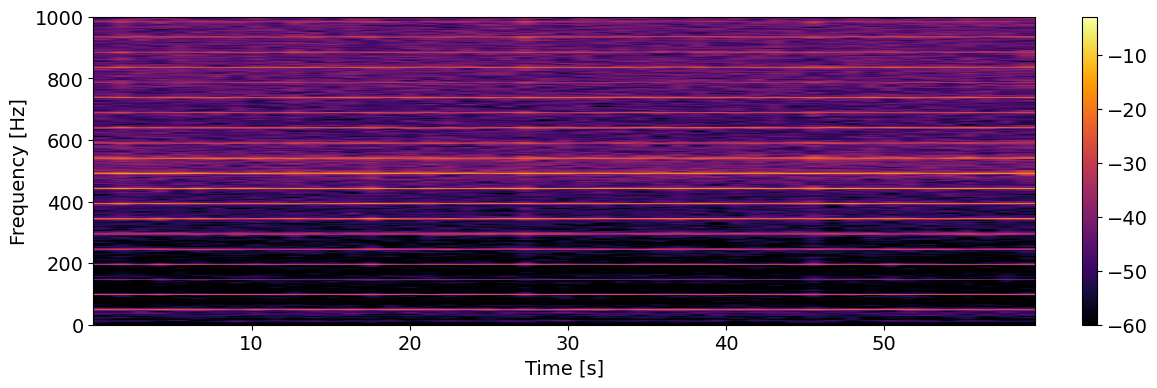
\includegraphics[width=\textwidth]{assets/results/time-frequency-spectrum/K3-z-STFT-1kHz.png}
        \caption{C1}
    \end{subfigure}
    \hfill
    \begin{subfigure}[b]{0.48\textwidth}
        \includegraphics[width=\textwidth]{assets/results/time-frequency-spectrum/M1-2-z-STFT-1kHz.png}
        \caption{M1-2}
    \end{subfigure}
    \hfill
    \begin{subfigure}[b]{0.48\textwidth}
        \includegraphics[width=\textwidth]{assets/results/time-frequency-spectrum/P1-3-z-STFT-1kHz.png}
        \caption{P1-3}
    \end{subfigure}
	\hfill
	\begin{subfigure}[b]{0.48\textwidth}
        \includegraphics[width=\textwidth]{assets/results/time-frequency-spectrum/P3-3-z-STFT-1kHz.png}
        \caption{P3-3}
    \end{subfigure}
    \caption{Machinery vibration spectrograms ($f_s$ = 26.8~kHz, $w$ = 8~kS)}
    \label{fig:evaluation:spectrograms}
\end{figure}

Spectrograms point out that under constant machine load, the significant frequencies stay more or less unchanged over time (Fig~\ref{fig:evaluation:spectrograms}). The resolution of the chart unit area is 306.95 ms and 3.26 Hz. Its magnitude is colored for decibel value. 

\begin{figure}[h]
    \centering
    \begin{subfigure}[b]{0.48\textwidth}
        \includegraphics[width=\textwidth]{assets/results/time-frequency-spectrum/P1-slow-down.png}
        \caption{P1 turns off ($w$ = 4~kS)}
    \end{subfigure}
    \hfill
    \begin{subfigure}[b]{0.48\textwidth}
        \includegraphics[width=\textwidth]{assets/results/time-frequency-spectrum/P2-speed-up.png}
        \caption{P2 turns on ($w$ = 32~kS)}
        \label{fig:evaluation-sigma-pump-interference}
    \end{subfigure}
    \caption{Vibrations of water pumps during switch over ($f_s$ = 26.8~kHz)}
    \label{fig:evaluation:pump-switch-over}
\end{figure}


The water pump switch on and off creates a fast change in shaft speed, which cannot be analyzed for resonance bands with enough time resolution by an automatic system at a chosen sampling rate. Due to inertia, slowing down takes about 10 seconds, whereas the speed up is half a second (Fig.~\ref{fig:evaluation:pump-switch-over}. The interference from excessive vibrations of the adjacent Sigma pump is picked up by the accelerometer on the KSB pump just before their switchover occurs (Fig~\ref{fig:evaluation-sigma-pump-interference}).

\begin{figure}[h]
    \centering
    \begin{subfigure}[b]{\textwidth}
        \includegraphics[width=\textwidth]{assets/results/feature-values/pumps-TD-dim-3.png}
        \caption{Time-domain features}
    \end{subfigure}
    \hfill
    \begin{subfigure}[b]{\textwidth}
        \includegraphics[width=\textwidth]{assets/results/feature-values/pumps-FD-dim-3.png}
        \caption{Frequency-domain features}
    \end{subfigure}
    \caption{The atrribute value ranges of Pump dataset}
\end{figure}

The range of feature values for compressors and pumps are higher than in MaFaulDa despite most of them describing baseline status (Fig~\ref{fig:evaluation-sigma-pump-interference}). The increses can be seen for example on the interquartile range of rms (7.33 - 14.62 $\mathrm{m/s}^2$), centroid (3806 - 6003 Hz) or entropy (9.40 - 13.22 nats).

\chapter{Conclusion} \label{section:conclusion}  
%TODO
% Furure work - more features from one recoding - in windows
% Different election methods and metrics
% Combine feature selection with incremntal learining
% Find other ML model also suitable HoeffdingTreeClassifier - losing original data for labeling - mechnaism of transforming samples to model represntatin

In the thesis we focused on trend indicator selection for an inexpensive industrial condition monitoring solution from vibration signals. The goal is to enable timely fault detection of machinery parts with as little input data as possible. For that purpose, we answer four research questions.

Attributes extracted to describe machine behavior come mainly from descriptive statistics, audio signal processing studies, and vibrodiagnostics technical standards (ISO 20186 and ISO 13343). These formulas compute 10 features summarizing the waveform in the temporal domain and 11 features characterizing spectral density estimation in 3 spatial directions \textbf{(RQ1)}.

In order to achieve more pronounced data savings, we choose the subset of 3 features in each domain by keeping the ones with the most similarity to the target variable. Feature selection metrics of the correlation coefficient, F statistic, mutual information, and their rank product are applicable in supervised learning. The features are squished from multiple dimensions using the Euclidian norm. Lossy compression ratios attained are 2381:1 for all features and 25000:1 for 6 features in the MaFaulDa dataset. We managed to discard more than 99.995\% of irrelevant data \textbf{(RQ2)}.

Feature subsets are subjected after normalization to a k-nearest neighbor classifier that ascertains their relative fault detection power. Because of model overtraining with small k, the feature triplets equal or slightly outperformed the whole set of features on the validation set with accuracy up to 10\%. The spectral features reach higher accuracies than temporal because of their smaller interdependency \textbf{(RQ3)}. 

The ensemble of feature selection with rank product produces the best model performance out of three combined in the majority of situations. No approach could find a triplet of predictors with an accuracy close to optimal one discovered exhaustively. Training on three principal components produced better accuracy than filtering feature selection, but PC mapping onto original trend indicators is unclear even in loading plots \textbf{(RQ3)}.

The considerable obstacle in an autonomous fault detection system deployment is the availability of labels for target variables. Annotations can be assigned belatedly or even never. Incremental learning k-NN model on an unbalanced dataset on the whole feature set achieves at best 90\% accuracy with immediate feedback, 85\% with labels coming in 250 long tumbling windows, and 82\% with just 25\% of observations associated with the label. The comparable model trained in batch reaches an accuracy of 98\% \textbf{(RQ4)}.

Conclusions so far have been made on the MaFaulDa dataset imitating the realistic conditions. Therefore, in proper validation of the proposed solution in practice, we will compare it with the custom-made dataset. 

The vibration signals will be gathered on compressors in air conditioning units and water pumps in municipal pumping stations. We will develop firmware for sensor units capable of sampling accelerometers and saving measurements onto SD cards. The challenge awaits us in labeling samples themselves as it requires substantial expert knowledge. 


%\nocite{*}
\printbibliography[heading=bibintoc]

%  Appendix ---------------------------------------------------------
\addtocontents{toc}{\protect\setcounter{tocdepth}{0}}
\addtocontents{toc}{\cftpagenumbersoff{chapter}}
\let\svaddcontentsline\addcontentsline
\renewcommand\addcontentsline[3]{%
  \ifthenelse{\equal{#1}{lof}}{}%
  {\ifthenelse{\equal{#1}{lot}}{}{\svaddcontentsline{#1}{#2}{#3}}}}

\appendix
\titleformat{\chapter}{\normalfont\LARGE\bf}{Appendix \thechapter:}{0.5em}{}
\renewcommand{\chaptermark}[1]{\markboth{\MakeUppercase{Appendix \thechapter.\ #1}}{}}

% Ak nechce vypísať čísla strán na konci prílohy: \cleardoublepage
\thispagestyle{empty}
\chapter{Resume}
\pagenumbering{arabic}
\renewcommand*{\thepage}{A-\arabic{page}}


\clearpage


\thispagestyle{empty}
\chapter{Technical documentation} \label{appendix:technical-docs}
\pagenumbering{arabic}
\renewcommand*{\thepage}{B-\arabic{page}}
The documentation contains a description of Jupyter Notebooks, Python package \verb|vibrodiagnostics| with utility functions for machine learning, and data logger firmware. Pages of \LaTeX \; documentation for Python were autogenerated by documentation tool \textbf{Sphinx}. Pages from C source code were created by \textbf{Doxygen}. 

\section{Jupyter notebooks}
\begin{itemize}[noitemsep]

\item \textbf{cluster-dbscan.ipynb} - The clustering feasibility of the DBSCAN algorithm in the MaFaulDa dataset. Experiments to find the best epsilon parameter for complete sets of time-domain and frequency-domain features. Epsilon is estimated by localizing the knee on the curve of nearest neighbours. The method turned out to be unreliable in separating different groups of fault types. The clustering produced too many or too few samples based on the choice of minimal samples.

\item \textbf{eda-bearing-faults.ipynb} - Mark the bearing characteristic frequencies in the frequency spectrum in the axis of motion for chosen recordings from the MaFaulDa dataset, scroll compressors, water pumps, and electric motors. The bearing frequencies are calculated from coefficients or physical dimensions for the bearing designation.

\item \textbf{eda-files.ipynb} - Time-domain vibration signal waveforms are charted for acceleration values and velocity after integration. Measurements are compared between fault types or measurement positions. Statistical tests for normality and stationarity of oscillations are conducted. Comparisons from all axes for peak finding MMS algorithm, cumulative frequency spectrum, and time-frequency spectrum. Orbitals of detected fundamental frequency are shown in the spatial graph. Options are to view signals for chosen files from the MaFaulDa dataset on the inner bearing, outer bearing, or for the Pumps industrial dataset.

\item \textbf{eda-ksb-cloud.ipynb} - Overall vibration rms velocities in hourly intervals for two identical water pumps are shown in ISO severity levels. Total running time is summed from periods when each pump has been operational. Frequency spectra are also compared but are proven to have too low resolution for any conclusive result in fault recognition.

\item \textbf{eda-pumps.ipynb} - It visualizes amplitude histograms and frequency spectrum of every time series in the Pump dataset next to one another.  Spectrograms of selected situations are depicted, such as rotation speed up or slow down. This notebook is instrumental in spotting patterns between different places and dates and checking for signal clipping.

\item \textbf{eda-standing-fan.ipynb} - Estimate the rotational speed of the standing fan based on the audio recording and compare it to the estimate from vibrations. The accelerometer is attached to the back, side, and front of the shaft.

\item \textbf{extraction-mafaulda.ipynb} - Feature extraction of a complete set of features from the entire MaFaulDa in time and frequency domain (TD and FD sets) to CSV files. Enable variable \emph{EXTRACT} to proceed with a lengthy calculation that takes around ten minutes for each set. When the extraction flag is disabled, the notebook loads the already extracted files with attributes.

\item \textbf{extraction-pumps.ipynb} - Feature extraction of a complete set of features from Pump datatset in time and frequency domain (TD and FD sets) to CSV files. Enable variable \emph{EXTRACT} to proceed with calculation.

\item \textbf{feature-summary.ipynb} - Count the occurrences of predictors in the best triplets over setup experimental conditions. Feature selection techniques produce bar charts with different orderings. The explained variance of complete feature sets is shown alongside the separability of clusters measured by silhouette score. This notebook generates CSV files of the best feature sets used in \emph{knn-batch.ipynb}.

\item \textbf{iit-src-paper.ipynb} - Run the experiments described in IIT.SRC 2024 paper in Appendix~\ref{appendix:iit-src-paper}. Set variables \emph{USE\_ONE\_AXIS} and \emph{MAFAULDA\_ LABEL\_METHOD} to one of the allowed options to generate all possible results. Running the experiments and not reading precomputing results requires enabling \emph{GENERATE} variable. Additionally, the hyperparameters of the model can be changed to tune the accuracy.

\item \textbf{knn-batch.ipynb} - Train k-NN classifiers with k = 5 on three members' best subsets of features found in \emph{feature-summary.ipynb}. Evaluate a wide range of performance metrics. Plot relation of k-neighbours on error rate for subset picked by the rank product method.

\item \textbf{knn-mafaulda.ipynb} - The results of the experiments are described in the Exploratory analysis of MaFaulDa and the evaluation chapter. The setup of experimental scenarios for batch and incremental learning is followed by scales of features and their correlations. Every combination of parameters put into k-NN is captured in graphs of accuracy. Feature selection methods are compared under experimental conditions. Incremental learning on subset combinations is carried out in the gradual evolution of relative fault severities.

\item \textbf{knn-online.ipynb} - Simulate incremental learning process for the complete feature sets. The source domain for features is chosen in variable \emph{DOMAIN}. The progressive valuation of k-NN accuracy compares situations with varied sliding windows and gaps between annotated observations. The performance at the end of the training is written in tables.

\item \textbf{wavelets.ipynb} - Features computed from wavelet packet coefficients are chosen and sorted using feature selection scores. The effect of varying the depth of decomposition is viewed in stacked plots. The difference in scores between feature coefficients is plotted in bar charts.
\end{itemize}

\section{Data analysis package}
\includepdf[pages=3-20,scale=0.9,clip,trim=0mm 20mm 0mm 20mm,pagecommand={}]{chapters/appendix/sphinx-vibrodiagnostics}

\section{Data logger firmware}
\includepdf[pages=2-10,scale=0.9,clip,trim=0mm 20mm 0mm 20mm,pagecommand={}]{chapters/appendix/doxygen-firmware}


\thispagestyle{empty}
\chapter{User Guide} \label{appendix:user-guide}
\pagenumbering{arabic}
\renewcommand*{\thepage}{C-\arabic{page}}

\section{Installation guide}
The development platform was Acer Aspire A515-47 laptop with Linux distribution \emph{Manjaro 23.1.4.} and kernel version 6.1. The installation process consists of getting the Python 3.11. packages for dataset analysis and development tools for building and flashing firmware for data logger. The paths are written relative to the root directory of the digital medium after unzipping.

The dependencies for running Jupyter notebooks can be installed by simply executing the following command ideally under a Python virtual environment:
\begin{lstlisting}[style=messages]
$ pip install -r docs/requirements.txt
\end{lstlisting}

To run the Jupyter environment and view notebooks run:
\begin{lstlisting}[style=messages]
$ jupyter lab
\end{lstlisting}

Building and uploading firmware of the data logger demands the following to be installed:
\begin{enumerate}
\item {Install system prerequisites and download ESP-IDF:
\begin{lstlisting}[style=messages]
$ sudo pacman -S --needed gcc git make flex bison gperf python cmake ninja ccache dfu-util libusb
$ mkdir -p ~/esp
$ cd ~/esp
$ git clone -b v5.2.1 --recursive https://github.com/espressif/esp-idf.git
\end{lstlisting}}

\item {Install the tools used by ESP-IDF which are compiler, debugger, etc:
\begin{lstlisting}[style=messages]
$ cd ~/esp/esp-idf
$ ./install.sh esp32
\end{lstlisting}}

\item {
Connect ESP32 microcontroller via USB and flash firmware onto the device:
\begin{lstlisting}[style=messages]
$ . ~/esp/esp-idf/esp-idf/export.sh
$ cd firmware
$ idf.py build
$ idf.py -p /dev/ttyUSB0 flash
\end{lstlisting}}
\end{enumerate}

\section{Data logger guide}
To measure vibrations with a data logger follow these steps.

\begin{enumerate}[noitemsep]
\item Insert empty microSD card to the data logger.
\item Attach the accelerometer sensor to the surface of measurement.
\item Press the button and watch the LED light up.
\item When the light turns off sooner before the minute mark, the buffer was dropped, and the final file can be incomplete.
\item Wait until the LED turns off, the recording is saved to file numbered sequentially from \emph{1.tsv} upwards.
\item {Move files from microSD card to a separate directory e.g. \emph{abc} and run for conversion to tsv files:
\begin{lstlisting}[style=messages]
$ python bin2tsv.py abc 4
\end{lstlisting}}
\end{enumerate}


\section{Documentation guide}
Built documentation is located in directory \emph{docs} of the digital medium. It can be rebuild using documentation tools \emph{Doxygen} for firmware C source code and \emph{Sphinx} for data analysis Python code. The steps of generating documentation from souce codes are as follows.

\begin{enumerate}[noitemsep]
\item {Install necessary documentation tools:
\begin{lstlisting}[style=messages]
$ sudo pacman -S doxygen
$ pip install sphinx sphinx-rtd-theme sphinx_autodoc_defaultargs
\end{lstlisting}}
\item {Rebuild the documentation using Doxygen and Sphinx:
\begin{lstlisting}[style=messages]
$ doxygen docs/firmware/doxygen.conf
$ cd docs/vibrodiagnostics
$ make html
\end{lstlisting}}
\item {View Doxygen docs in \emph{docs/firmware/html/topics.html} and Sphinx docs in \emph{docs/vibrodiagnostics/build/html/index.html}}
\end{enumerate}

\thispagestyle{empty}
\chapter{IIT.SRC 2024 Paper} \label{appendix:iit-src-paper}
\pagenumbering{arabic}
\renewcommand*{\thepage}{D-\arabic{page}}

\thispagestyle{empty}
\includepdf[pages=-, scale=1, pagecommand={}]{chapters/appendix/iit-src-paper}


\thispagestyle{empty}
\chapter{Work plan}
\pagenumbering{arabic}
\renewcommand*{\thepage}{E-\arabic{page}}

\section{Summer semester - DP1}

\begin{table}[h!]
\def\arraystretch{1.25}
\begin{tabular}{|l|p{12cm}|}
\hline
\textbf{Period} & \textbf{Work}                                                                                                                                                                                                                         \\ \hline
\nth{1} week         & Consultation with the supervisor on directions of the future work based on literature review during the previous semester.
\\ \hline
\nth{2} week         & Outline the key sections of the analysis part in the thesis.
\\ \hline
\nth{3} week         & Match supporting literature with analysis sections. Further investigation on the feature engineering methodology in CbM.
 \\ \hline
\nth{4} week         & Summarize notes from condition monitoring articles and video recordings of tutorials and conferences.
 \\ \hline
\nth{5} week         & Research transformation of a vibration signal to feature space using time-frequency, harmonic, and energy statistical metrics. Progress report meeting with the supervisor.
 \\ \hline
\nth{6} week         & Find articles and take notes about unsupervised and semi-supervised techniques in streaming data for machinery diagnostics.
 \\ \hline
\nth{7} week         & Narrow down a wide variety of applicable methods for signal decomposition.
 \\ \hline
 \nth{8} week         & Exploratory analysis on evaluation datasets. Progress report meeting with the supervisor on the topic of related work.
 \\ \hline
 \nth{9} week         & Organize detailed outline out of notes gathered during literature research. 
 \\ \hline
  \nth{10} week         & Write up the problem analysis about condition monitoring and evaluation datasets.
 \\ \hline
  \nth{11} week         & Write up the analysis section about feature engineering.
 \\ \hline
  \nth{12} week         & Write up the analysis section about machine learning diagnostics and consult the final choice of methods in the analysis section.
 \\ \hline
\end{tabular}
\end{table}

\clearpage
\newpage
\section{Winter semester - DP2}

\begin{table}[h!]
\def\arraystretch{1.25}
\begin{tabular}{|l|p{12cm}|}
\hline
\textbf{Period} & \textbf{Work}                                                                                                                                                                                                                         \\ \hline
\nth{1} week         & Semester kickoff meeting to set goals, and experiments and discuss the status of collaborations with partners.
\\ \hline
\nth{2} week         &  Arrange collaboration with an alternative industry partner. Prepare a checklist for the technical inspection of machinery. Construct a device for exploratory measurements.
\\ \hline
\nth{3} week         & Technical inspection of air conditioning units in the data center. Feature extraction step to calculate features from MaFaulDa.
 \\ \hline
\nth{4} week         & Consultation about the plan for a machine to measure in the data center and a better device for measurement.
 \\ \hline
\nth{5} week         &  In feature selection using various metrics to determine sets of best features in the MaFaulDa.
 \\ \hline
\nth{6} week         & Feature selection used in k-NN multiclass and binary classificator.
 \\ \hline
\nth{7} week         & Explore incremental learning k-NN algorithm with MaFaulDa dataset. Consultation and status report.
 \\ \hline
 \nth{8} week         & Shorten analysis chapter about wavelets. Look at clustering detection incremental learning in MaFaulDa.
 \\ \hline
 \nth{9} week         &  Refactor separate trials in feature selection to integrate them into the pipeline for k-NN validation. Consultation to discuss progress.
 \\ \hline
  \nth{10} week         & Include incremental learning in analysis. Experiment with gradual feature selection in incremental learning.
 \\ \hline
  \nth{11} week         & Consultation in preparation for machine inspections. Preliminary measurements of fan, compressors, and pump. Design the firmware for the new datalogger.
 \\ \hline
  \nth{12} - \nth{15} week         &  Write up design chapter: research questions and visualization export. Finish writing a chapter on design and implementation.
 \\ \hline
\end{tabular}
\end{table}

The semester for DP2 was split into 3 periods. Feature engineering and ML model evaluation was planned from \nth{1} to \nth{4} week, and technical inspections and plan of measurement in weeks \nth{4} to \nth{8}.

In reality, these tasks switched order because, between \nth{1} to \nth{5} week, we needed to acquire alternative partner and check their machiners for viability in our study. Only then since \nth{4} until \nth{11} week, the main focus was on experiments with the MaFaulDa. 

Lastly, preliminary measurements were conducted, as was the plan. The requirements were presented for the new sensor device and its firmware.
\clearpage
\newpage

\section{Summer semester - DP3}
\begin{table}[h!]
\def\arraystretch{1.25}
\begin{tabular}{|l|p{12cm}|}
\hline
\textbf{Period} & \textbf{Work}                                                                                                                                                                                                                         \\ \hline
\nth{1} week  & Build and debug hardware of data logger with the consultant. 
\\ \hline
\nth{2} week & Implement and test firmware on standing fan for logging signal to SD card.
\\ \hline
\nth{3} week & First compressor (\nth{20} February) and water pump (\nth{27} and \nth{28} February) vibration measurements and their fault and frequency analysis. 
 \\ \hline
\nth{4} week & Replace two time-domain features and evaluate on MaFaulDa and own dataset. Repeated measurement of compressors (\nth{5} March).
 \\ \hline
\nth{5} week & Perform PCA analysis of whole feature sets. Consultation about methods for own dataset evaluation.
 \\ \hline
\nth{6} week  & Consultation with experts in SjF STU. Formulate research goals for scientific paper and create graphs of the model results. Experiment with the k-value and number of features to reach better accuracy. Repeated measurement of compressors (\nth{19} March).
 \\ \hline
\nth{7} week & Repeated measurement of water pumps (\nth{26} and \nth{27} March). Request and download data about pumps from KSB Cloud.
 \\ \hline
 \nth{8} week & Write up complete paper and submit to IIT.SRC student conference after feedback from supervisor.
 \\ \hline
 \nth{9} week & Refactor Jupyter notebooks and apply different labeling strategies applied in paper to incremental learning.
 \\ \hline
  \nth{10} - \nth{13} week & Update design chapter and finish text according to figures generated by experiments.
 \\ \hline
\end{tabular}
\end{table}

The final semester aimed at gathering dataset from compressors and water pumps with the accelerometer data logger. The k-NN model was validated with different hyperparameters. The data collection finished sooner in \nth{7} week whereas originally it was planned until \nth{10} week because it became apparent that during a such short period, the change in machine vibrations would be negligible. The preparation for IIT.SRC conference was also not originally planned and took time away from finishing the thesis.

\clearpage


\thispagestyle{empty}
\setcounter{figure}{0}
\chapter{Digital medium}
\pagenumbering{arabic}
\renewcommand*{\thepage}{E-\arabic{page}}
\par Registration number of thesis in AiS: \RegNo
\par Contents of the digital medium:
\par Name of submitted archive directory: DP\_MiroslavHajek.zip
\par Notice: Digital medium has more than 1 GiB and is available to the thesis supervisor.
\par The MaFaulDa dataset is publically available at: \url{https://www02.smt.ufrj.br/~offshore/mfs/database/mafaulda/full.zip}

\begin{itemize}[noitemsep]
\item[\textbf{>}] \textbf{datasets} - raw vibration data from machinery, and reports that took long to calculate.
	\begin{itemize}[noitemsep]
	\item[\textbf{>}] \textbf{FluidPump.zip} - custom recorded dataset of vibrations from air compressors and water pumps
	\item[\textbf{>}] \emph{MAFAULDA.zip} - placeholder where the downloaded MaFaulDa dataset should be placed
	\item[\textbf{>}] \textbf{best-subset} - the subset of features chosen to three-member subsets most frequently
	\item[\textbf{>}] \textbf{features} - features extracted from datasets in multiple domains
	\item[\textbf{>}] \textbf{ksb-cloud} - data exported from KSB cloud monitoring of vibration rms velocity and frequency waveform for chosen dates.
	\item[\textbf{>}] \textbf{misc-fluid-pump} - other non-standard measurements from pumps such as during speed up, slow down, or noise.
	\item[\textbf{>}] \textbf{knn-accuracy-distribution} - 
	\item[\textbf{>}] \textbf{knn-incremental-accuracy} - The incremental k-NN model accuracy after each sample for various lengths of tumbling window and gaps between labels 
	\item[\textbf{>}] \textbf{standing-fan} - audio for an estimate of fan rotational speed and measurements done in firmware verification on the back, side, and front of the fan.
	\end{itemize}
\item[\textbf{>}] \textbf{docs} - the documentation generated from source code comments  using automated tool
	\begin{itemize}[noitemsep]
	\item[\textbf{>}] \textbf{html-notebooks} - export of Jupyter notebooks for all basic configurations in HTML format
	\item[\textbf{>}] \textbf{doxygen} - documentation of \emph{firmware} 
	\item[\textbf{>}] \textbf{sphinx} - documentation of \emph{vibrodiagnostics} package
	\end{itemize}
\item[\textbf{>}] \textbf{firmware} - source code in \emph{main} directory for accelerometer data logger firmware written in C language with ESP-IDF SDK. The script \emph{bin2tsv.py} converts files saved to SD card in binary format to a tsv file.
\item[\textbf{>}] \textbf{notebooks} - Jupyter notebooks for data exploration, data analysis, and machine learning on provided datasets
\item[\textbf{>}] \textbf{vibrodiagnostics} - Python package of commonly used function in Jupyter notebooks for data processing
\end{itemize}

\end{document}
